%!TEX root=tese.tex
\chapter{Determinação da concentração mássica de células para efetuar a lise}
\label{app:1}
Para determinar a concentração mássica de células (peso húmido) a usar na etapa de lise foram realizados ensaios prévios de estabilidade de lisados. Para isso, efetuou-se a lise alcalina de suspensões de células com diferentes concentrações mássicas (figura~\ref{fig:estabilidade_lisados}). A concentração mássica foi determinada como o rácio entre o peso húmido de células e o volume de tampão usado na sua ressuspensão. Os lisados obtidos foram posteriormente processados por centrifugação para remover o conteúdo sólido formado durante a lise. Como se pode verificar na figura~\ref{fig:estabilidade_lisados}, para as concentrações de 180 e 240 g/L, observa-se um aumento da densidade ótica dos lisados centrifugados ao longo do tempo, facto que indica a ocorrência da precipitação de algum do material inicialmente dissolvido. Optou-se por escolher a concentração de 120\,g/L, para a qual se verificou um reduzido aumento da densidade ótica, estando este valor igualmente dentro da gama de concentrações usadas por outros autores \cite{theo,chamsart,urthaler}. Com a escolha deste valor de concentração pretende-se assim evitar a ocorrência da precipitação de alguns constituintes do lisado em operações subsequentes à etapa da lise alcalina, facto que poderia introduzir efeitos indesejados na interpretação e desempenho dos processos.
\index{concentração!mássica de células}
\index{peso húmido}
\index{lisado!estabilidade} 
\begin{figure}[!h]
    \centering
    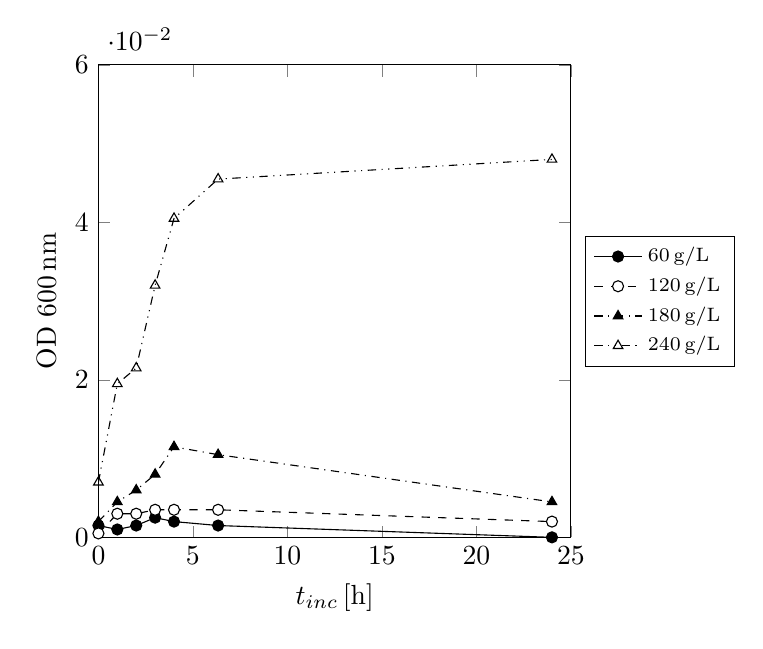
\begin{tikzpicture}

\begin{axis}[
	width=6cm,
	height=6cm,
	scale only axis,
	xmin=0,
	xmax=25,
	xlabel={$t_{\mr{inc}}$\,[h]},
	ymin=0,
	ymax=0.06,
	ylabel={OD 600\,nm},
	ylabel near ticks,
	at={(0cm,0cm)},
	anchor=south west,
	legend style={at={(1.03,0.5)},legend columns=1,anchor=west,font=\scriptsize,draw=black,fill=white,legend cell align=left}
	]
\addplot[
color=black,
solid,
mark=*,
mark options={solid,fill=black,draw=black}
]
table[row sep=crcr]{
0.000000 0.001500\\
1.000000 0.001000\\
2.000000 0.001500\\
3.000000 0.002500\\
4.000000 0.002000\\
6.333333 0.001500\\
24.00000 0.000000\\
};\addlegendentry{60\,g/L};

\addplot[
color=black,
dashed,
mark=*,
mark options={solid,fill=white,draw=black}
]
table[row sep=crcr]{
0.000000 0.000500\\
1.000000 0.003000\\
2.000000 0.003000\\
3.000000 0.003500\\
4.000000 0.003500\\
6.333333 0.003500\\
24.00000 0.002000\\
};\addlegendentry{120\,g/L};

\addplot[
color=black,
dashdotted,
mark=triangle*,
mark options={solid,fill=black,draw=black}
]
table[row sep=crcr]{
0.000000 0.002000\\
1.000000 0.004500\\
2.000000 0.006000\\
3.000000 0.008000\\
4.000000 0.011500\\
6.333333 0.010500\\
24.00000 0.004500\\
};\addlegendentry{180\,g/L};

\addplot[
color=black,
dashdotdotted,
mark=triangle,
mark options={solid,fill=white,draw=black}
]
table[row sep=crcr]{
0.000000 0.007000\\
1.000000 0.019500\\
2.000000 0.021500\\
3.000000 0.032000\\
4.000000 0.040500\\
6.333333 0.045500\\
24.00000 0.048000\\
};\addlegendentry{240\,g/L};

\end{axis}

\end{tikzpicture}
    \caption[Densidade ótica de lisados em função do tempo de incubação]{Variação da densidade ótica (600\,nm) em função do tempo de incubação para lisados alcalinos centrifugados a diferentes valores de concentração mássica de células (peso húmido).}
    \label{fig:estabilidade_lisados}
\end{figure}

\chapter{Caracterização de lisados centrifugados}
\label{app:2}
Foram utilizados dois géis de SEC diferentes: o gel Sephacryl S-1000 SF e o gel Sephacryl S-100 HR (\emph{GE Healthcare}), estando as suas principais características indicadas na tabela~\ref{tab:sephacryl}.\index{Sephacryl S-1000!características}\index{Sephacryl S-100!características} 
\begin{table}
\caption[Principais características dos géis Sephacryl S-100 HR e Spehacryl S-1000 SF]{Principais características dos géis Sephacryl S-100 HR e Spehacryl S-1000 SF \cite{sec}.}
\label{tab:sephacryl}
\begin{tabularx}{\textwidth}{Y Y Y Y Y} 
 \toprule
Gel & Intervalo de fracionamento [kDa] & Capacidade & Caudal recomendado & Tamanho médio das partículas \\
 \midrule  
Sephacryl \newline S-100 HR & 1--100 & 0.4\%--4\% do volume total de coluna & 10--35\,cm/h & 47\,\micro m \\
Sphacryl \newline S-1000 SF & $500-5\times 10^{5}$ & 0.4\%--4\% do volume total de coluna & 2--30\,cm/h & 65\,\micro m \\
\bottomrule 
\end{tabularx}
\end{table}

Para efetuar a análise de lisados por SEC, os géis foram empacotados numa coluna com 50\,mL de volume (\emph{Sigma}), segundo as recomendações do fabricante. Obteve-se no final um volume de gel de aproximadamente 46\,mL. A coluna foi conectada a um sistema cromatográfico (Äkta purifier, \emph{GE Healthcare}) e as amostras de lisado foram injetadas e eluídas a um caudal de 0.5\,mL/min, usando tampão Tris/HCl 10\,mM a pH 8.00, com 150\,mM de NaCl, como eluente. A absorvância do eluato foi continuamente monitorizada a 260\,nm. Em alguns ensaios foram recolhidas amostras do eluído em intervalos de 10\,min. Estas amostras foram posteriormente analisadas por AGE, HIC e BCA.\index{coluna cromatográfica}\index{AGE}\index{BCA}\index{akta@Äkta}

Na figura~\ref{fig:s1000} encontra-se o resultado da análise do lisado de \pVAX\ no gel Sephacryl S-1000 SF. No cromatograma obtido (figura~\ref{fig:s1000}~a) é possível identificar dois picos parcialmente sobrepostos. No primeiro pico elui o plasmídeo, que essencialmente é recolhido nas frações 4 e 5 (figura~\ref{fig:s1000}~c). Devido à existência no lisado de várias espécies de RNA, estas biomoléculas eluem ao longo do segundo pico, com a prevista tendência da redução de tamanhos ao longo das várias frações. Nas análises de HIC das frações selecionadas (figura~\ref{fig:s1000}~b), verifica-se a presença de plasmídeo apenas na fração 5. A área do pico na região 3 (contaminantes hidrofóbicos) diminui ao longo das frações, e na fração 10, que já parece não conter RNA, é nula. Na região 2 (contaminantes hidrofílicos), observa-se uma tendência contrária, registando-se uma maior absorvância na fração 9. Este facto parece indicar que os compostos que eluem na região 2 apresentam uma menor massa molecular.\index{cromatograma}\index{SEC!cromatograma}\index{lisado!SEC}\index{DNA plasmídico!SEC}\index{RNA!SEC}
\begin{figure}[!t]
    \centering
    \begin{tikzpicture}[scale = 0.9]
%\draw[help lines] (0cm, 0cm) grid (17cm, 14cm);

\node[font = \large, below] at (1.5, 14) {a)};
\node[font = \large, below] at (1.5, 8.5) {b)};
\node[font = \large, below] at (1.5, 2.5) {c)};

\draw (12.1, 1.2) -- (12.25, 1.2) -- (12.35, 1.6) -- (12.5, 1.6)  node[right] {pDNA\,(oc)};
\draw (12.1, 1) -- (12.5, 1) node[right] {pDNA\,(sc)};
\draw (12.1, -0.1) -- (12.5, -0.1) node[right] {HMw\,RNA};
\draw (12.1, -0.75) -- (12.5, -0.75) node[right] {LMw\,RNA};

\node[
below right,
align = right
] at (10.75, 13.75) {Sephacryl \\ S-1000 SF};

\node[below left, font = \scriptsize] at (4, 7) {HIC};
\node[below left, font = \scriptsize] at (8, 7) {HIC};
\node[below left, font = \scriptsize] at (12, 7) {HIC};
\node[below left, font = \scriptsize] at (16, 7) {HIC};

\draw[dashed] (4.7, 9) -- (4.7, 10);
\node[above, font = \scriptsize] at (4.95, 10) {1};
\draw[dashed] (5.2, 9) -- (5.2, 10);
\node[above, font = \scriptsize] at (5.45, 10) {2};
\draw[dashed] (5.699, 9) -- (5.699, 10);
\node[above, font = \scriptsize] at (5.95, 10) {3};
\draw[dashed] (6.199, 9) -- (6.199, 10);
\node[above, font = \scriptsize] at (6.45, 10) {4};
\draw[dashed] (6.699, 9) -- (6.699, 10);
\node[above, font = \scriptsize] at (6.95, 10) {5};
\draw[dashed] (7.199, 9) -- (7.199, 10);
\node[above, font = \scriptsize] at (7.45, 10) {6};
\draw[dashed] (7.699, 9) -- (7.699, 10);
\node[above, font = \scriptsize] at (7.95, 10) {7};
\draw[dashed] (8.199, 9) -- (8.199, 10);
\node[above, font = \scriptsize] at (8.45, 10) {8};
\draw[dashed] (8.699, 9) -- (8.699, 10);
\node[above, font = \scriptsize] at (8.95, 10) {9};
\draw[dashed] (9.199, 9) -- (9.199, 10);
\node[above, font = \scriptsize] at (9.45, 10) {10};
\draw[dashed] (9.699, 9) -- (9.699, 10);
\node[above, font = \scriptsize] at (9.95, 10) {11};
\draw[dashed] (10.199, 9) -- (10.199, 10);

\draw[dashed] (6.699, 9) -- (1, 7) (7.199, 9) -- (4, 7);
\draw[dashed] (7.699, 9) -- (5, 7) (8.199, 9) -- (8, 7);
\draw[dashed] (8.699, 9) -- (9, 7) (9.199, 9) -- (12, 7);
\draw[dashed] (9.199, 9) -- (13, 7) (9.699, 9) -- (16, 7);

\begin{axis}[%
xlabel style = {fill = white},
x tick label style = {fill = white},
width=9cm,
height=5cm,
scale only axis,
xmin=-5,
xmax=85,
xlabel={$V_{\mr{R}}$\,[mL]},
% ymin=-500,
% ymax=3000,
ylabel={Absorvância 260\,nm [AU]},
at={(4cm, 9cm)},
anchor=south west,
% legend style={at={(1.03,0.5)},legend columns=1,anchor=west,font=\scriptsize,draw=black,fill=white,legend cell align=left}
]
\addplot[
color=black,
solid
]
table[row sep=crcr]{
0.000000 0.000005\\
0.080000 -0.000012\\
0.160000 0.000005\\
0.240000 0.000059\\
0.320000 0.000017\\
0.400000 0.000023\\
0.480000 -0.000002\\
0.560000 0.000060\\
0.640000 0.000044\\
0.720000 0.000039\\
0.800000 0.000035\\
0.880000 0.000059\\
0.960000 0.000075\\
1.040000 0.000104\\
1.120000 0.000095\\
1.200000 0.000111\\
1.280000 0.000095\\
1.360000 0.000057\\
1.440000 0.000107\\
1.520000 0.000103\\
1.600000 0.000046\\
1.680000 0.000048\\
1.760000 0.000120\\
1.840000 0.000120\\
1.920000 0.000129\\
2.000000 0.000183\\
2.080000 0.000143\\
2.160000 0.000135\\
2.240000 0.000152\\
2.320000 0.000160\\
2.400000 0.000169\\
2.480000 0.000147\\
2.560000 0.000194\\
2.640000 0.000182\\
2.720000 0.000199\\
2.800000 0.000187\\
2.880000 0.000206\\
2.960000 0.000218\\
3.040000 0.000225\\
3.120000 0.000284\\
3.200000 0.000272\\
3.280000 0.000303\\
3.360000 0.000301\\
3.440000 0.000318\\
3.520000 0.000301\\
3.600000 0.000306\\
3.680000 0.000301\\
3.760000 0.000320\\
3.840000 0.000331\\
3.920000 0.000276\\
4.000000 0.000310\\
4.080000 0.000267\\
4.160000 0.000336\\
4.240000 0.000333\\
4.320000 0.000298\\
4.400000 0.000313\\
4.480000 0.000383\\
4.560000 0.000355\\
4.640000 0.000422\\
4.720000 0.000438\\
4.800000 0.000422\\
4.880000 0.000442\\
4.960000 0.000490\\
5.040000 0.000476\\
5.120000 0.000474\\
5.200000 0.000459\\
5.280000 0.000442\\
5.360000 0.000481\\
5.440000 0.000469\\
5.520000 0.000481\\
5.600000 0.000439\\
5.680000 0.000495\\
5.760000 0.000536\\
5.841000 0.000485\\
5.921000 0.000528\\
6.001000 0.000499\\
6.081000 0.000539\\
6.161000 0.000575\\
6.241000 0.000599\\
6.321000 0.000559\\
6.401000 0.000599\\
6.481000 0.000593\\
6.561000 0.000581\\
6.641000 0.000623\\
6.721000 0.000642\\
6.801000 0.000636\\
6.881000 0.000636\\
6.961000 0.000643\\
7.041000 0.000668\\
7.121000 0.000605\\
7.201000 0.000655\\
7.281000 0.000658\\
7.361000 0.000641\\
7.441000 0.000681\\
7.521000 0.000636\\
7.601000 0.000685\\
7.681000 0.000694\\
7.761000 0.000664\\
7.841000 0.000684\\
7.921000 0.000750\\
8.001000 0.000756\\
8.081000 0.000759\\
8.161000 0.000759\\
8.241000 0.000778\\
8.321000 0.000777\\
8.401000 0.000780\\
8.481000 0.000821\\
8.561000 0.000790\\
8.641000 0.000817\\
8.721000 0.000820\\
8.801000 0.000808\\
8.881000 0.000800\\
8.961000 0.000828\\
9.041000 0.000815\\
9.121000 0.000818\\
9.201000 0.000810\\
9.281000 0.000805\\
9.361000 0.000759\\
9.441000 0.000729\\
9.521000 0.000733\\
9.601000 0.000759\\
9.681000 0.000773\\
9.761000 0.000719\\
9.841000 0.000752\\
9.921000 0.000747\\
10.001000 0.000761\\
10.081000 0.000743\\
10.161000 0.000772\\
10.241000 0.000800\\
10.321000 0.000828\\
10.401000 0.000803\\
10.481000 0.000799\\
10.561000 0.000806\\
10.641000 0.000872\\
10.721000 0.000835\\
10.801000 0.000841\\
10.881000 0.000886\\
10.961000 0.000870\\
11.041000 0.000905\\
11.121000 0.000924\\
11.201000 0.000942\\
11.281000 0.000974\\
11.361000 0.000968\\
11.441000 0.000999\\
11.521000 0.001064\\
11.601000 0.001090\\
11.681000 0.001165\\
11.761000 0.001267\\
11.841000 0.001266\\
11.921000 0.001366\\
12.001000 0.001408\\
12.081000 0.001464\\
12.161000 0.001530\\
12.241000 0.001664\\
12.321000 0.001752\\
12.401000 0.001932\\
12.481000 0.001998\\
12.561000 0.002184\\
12.641000 0.002308\\
12.721000 0.002368\\
12.801000 0.002537\\
12.881000 0.002776\\
12.961000 0.002944\\
13.041000 0.003114\\
13.121000 0.003309\\
13.201000 0.003526\\
13.281000 0.003781\\
13.361000 0.003993\\
13.441000 0.004228\\
13.521000 0.004460\\
13.601000 0.004752\\
13.681000 0.005081\\
13.761000 0.005402\\
13.841000 0.005729\\
13.921000 0.006023\\
14.001000 0.006396\\
14.081000 0.006765\\
14.161000 0.007122\\
14.241000 0.007506\\
14.321000 0.007924\\
14.401000 0.008374\\
14.481000 0.008765\\
14.561000 0.009189\\
14.641000 0.009614\\
14.721000 0.010167\\
14.801000 0.010645\\
14.881000 0.011172\\
14.961000 0.011720\\
15.041000 0.012226\\
15.121000 0.012800\\
15.201000 0.013239\\
15.281000 0.013757\\
15.361000 0.014426\\
15.441000 0.015032\\
15.521000 0.015725\\
15.601000 0.016355\\
15.681000 0.017069\\
15.761000 0.017805\\
15.841000 0.018597\\
15.921000 0.019551\\
16.001000 0.020516\\
16.081000 0.021565\\
16.161000 0.022731\\
16.241000 0.023994\\
16.321000 0.025354\\
16.401000 0.026753\\
16.481000 0.028372\\
16.561000 0.030074\\
16.641000 0.031818\\
16.721000 0.033666\\
16.801000 0.035852\\
16.881000 0.037998\\
16.961000 0.040450\\
17.041000 0.042975\\
17.121000 0.045647\\
17.201000 0.048442\\
17.281000 0.051314\\
17.362000 0.054437\\
17.442000 0.057514\\
17.522000 0.060843\\
17.602000 0.064287\\
17.682000 0.067693\\
17.762000 0.071273\\
17.842000 0.074854\\
17.922000 0.078307\\
18.002000 0.081988\\
18.082000 0.085662\\
18.162000 0.089341\\
18.242000 0.093134\\
18.322000 0.096862\\
18.402000 0.100664\\
18.482000 0.104379\\
18.562000 0.108152\\
18.642000 0.111869\\
18.722000 0.115485\\
18.802000 0.119244\\
18.882000 0.122869\\
18.962000 0.126471\\
19.042000 0.129987\\
19.122000 0.133456\\
19.202000 0.136792\\
19.282000 0.140135\\
19.362000 0.143286\\
19.442000 0.146427\\
19.522000 0.149424\\
19.602000 0.152369\\
19.682000 0.155072\\
19.762000 0.157708\\
19.842000 0.160218\\
19.922000 0.162543\\
20.002000 0.164872\\
20.082000 0.166962\\
20.162000 0.168887\\
20.242000 0.170697\\
20.322000 0.172500\\
20.402000 0.173922\\
20.482000 0.175223\\
20.562000 0.176511\\
20.642000 0.177732\\
20.722000 0.178730\\
20.802000 0.179755\\
20.882000 0.180319\\
20.962000 0.181033\\
21.042000 0.181499\\
21.122000 0.181875\\
21.202000 0.182221\\
21.282000 0.182391\\
21.362000 0.182432\\
21.442000 0.182397\\
21.522000 0.182230\\
21.602000 0.181921\\
21.682000 0.182067\\
21.762000 0.181346\\
21.842000 0.180976\\
21.922000 0.180700\\
22.002000 0.180109\\
22.082000 0.179598\\
22.162000 0.178928\\
22.242000 0.178142\\
22.322000 0.177539\\
22.402000 0.176854\\
22.482000 0.176046\\
22.562000 0.175331\\
22.642000 0.174546\\
22.722000 0.173804\\
22.802000 0.173055\\
22.882000 0.172320\\
22.962000 0.171444\\
23.042000 0.170632\\
23.122000 0.169757\\
23.202000 0.168823\\
23.282000 0.168120\\
23.362000 0.167454\\
23.442000 0.166803\\
23.522000 0.166051\\
23.602000 0.165235\\
23.682000 0.164487\\
23.762000 0.163874\\
23.842000 0.163248\\
23.922000 0.162753\\
24.002000 0.162323\\
24.082000 0.161738\\
24.162000 0.161178\\
24.242000 0.160935\\
24.322000 0.160240\\
24.402000 0.160026\\
24.482000 0.159694\\
24.562000 0.159412\\
24.642000 0.159145\\
24.722000 0.159152\\
24.802000 0.159004\\
24.882000 0.159075\\
24.962000 0.159041\\
25.042000 0.159189\\
25.122000 0.159327\\
25.202000 0.159404\\
25.282000 0.159606\\
25.362000 0.159957\\
25.442000 0.160321\\
25.522000 0.160865\\
25.602000 0.161206\\
25.682000 0.161704\\
25.762000 0.162173\\
25.842000 0.162882\\
25.922000 0.163415\\
26.002000 0.163985\\
26.082000 0.164998\\
26.162000 0.165915\\
26.242000 0.166802\\
26.322000 0.167868\\
26.402000 0.168961\\
26.482000 0.169773\\
26.562000 0.170847\\
26.642000 0.171899\\
26.722000 0.173683\\
26.802000 0.174868\\
26.882000 0.176120\\
26.962000 0.177469\\
27.042000 0.178722\\
27.122000 0.180024\\
27.202000 0.181880\\
27.282000 0.183625\\
27.362000 0.185156\\
27.442000 0.187148\\
27.522000 0.188809\\
27.602000 0.190864\\
27.682000 0.192499\\
27.762000 0.194694\\
27.842000 0.196672\\
27.922000 0.199054\\
28.002000 0.200817\\
28.082000 0.203412\\
28.162000 0.205236\\
28.242000 0.207614\\
28.322000 0.209868\\
28.402000 0.212335\\
28.482000 0.215120\\
28.562000 0.217895\\
28.642000 0.220711\\
28.722000 0.223742\\
28.802000 0.225550\\
28.882000 0.228795\\
28.963000 0.232286\\
29.043000 0.235801\\
29.123000 0.238807\\
29.203000 0.242224\\
29.283000 0.245456\\
29.363000 0.249094\\
29.443000 0.252011\\
29.523000 0.256490\\
29.603000 0.260862\\
29.683000 0.264727\\
29.763000 0.269661\\
29.843000 0.274496\\
29.923000 0.278429\\
30.003000 0.283900\\
30.083000 0.289057\\
30.163000 0.294361\\
30.243000 0.300178\\
30.323000 0.306302\\
30.403000 0.311713\\
30.483000 0.317856\\
30.563000 0.324377\\
30.643000 0.331720\\
30.723000 0.339276\\
30.803000 0.346555\\
30.883000 0.353924\\
30.963000 0.361804\\
31.043000 0.369969\\
31.123000 0.378329\\
31.203000 0.388228\\
31.283000 0.397598\\
31.363000 0.407558\\
31.443000 0.417180\\
31.523000 0.427861\\
31.603000 0.438171\\
31.683000 0.449574\\
31.763000 0.461711\\
31.843000 0.473982\\
31.923000 0.486644\\
32.003000 0.500019\\
32.083000 0.513435\\
32.163000 0.527285\\
32.243000 0.541708\\
32.323000 0.557082\\
32.403000 0.572698\\
32.483000 0.588997\\
32.563000 0.605621\\
32.643000 0.622405\\
32.723000 0.640522\\
32.803000 0.658602\\
32.883000 0.677050\\
32.963000 0.696308\\
33.043000 0.716060\\
33.123000 0.735988\\
33.203000 0.756768\\
33.283000 0.777807\\
33.363000 0.799078\\
33.443000 0.820978\\
33.523000 0.843283\\
33.603000 0.866371\\
33.683000 0.889995\\
33.763000 0.913564\\
33.843000 0.938195\\
33.923000 0.963037\\
34.003000 0.987637\\
34.083000 1.013363\\
34.163000 1.039300\\
34.243000 1.065809\\
34.323000 1.092339\\
34.403000 1.119232\\
34.483000 1.146312\\
34.563000 1.172731\\
34.643000 1.201148\\
34.723000 1.229689\\
34.803000 1.256619\\
34.883000 1.284750\\
34.963000 1.314427\\
35.043000 1.341273\\
35.123000 1.372002\\
35.203000 1.402077\\
35.283000 1.429478\\
35.363000 1.459628\\
35.443000 1.487945\\
35.523000 1.517103\\
35.603000 1.547431\\
35.683000 1.577236\\
35.763000 1.605070\\
35.843000 1.634496\\
35.923000 1.664224\\
36.003000 1.690402\\
36.083000 1.720217\\
36.163000 1.748883\\
36.243000 1.775655\\
36.323000 1.802405\\
36.403000 1.831752\\
36.483000 1.856150\\
36.563000 1.883565\\
36.643000 1.910656\\
36.723000 1.935716\\
36.803000 1.963200\\
36.883000 1.987332\\
36.963000 2.010419\\
37.043000 2.034161\\
37.123000 2.055421\\
37.203000 2.076349\\
37.283000 2.096337\\
37.363000 2.111922\\
37.443000 2.128489\\
37.523000 2.145931\\
37.603000 2.162190\\
37.683000 2.181368\\
37.763000 2.195936\\
37.843000 2.211330\\
37.923000 2.227933\\
38.003000 2.244843\\
38.083000 2.262054\\
38.163000 2.275220\\
38.243000 2.291927\\
38.323000 2.301516\\
38.403000 2.312062\\
38.483000 2.324588\\
38.563000 2.330830\\
38.643000 2.342349\\
38.723000 2.351656\\
38.803000 2.363496\\
38.883000 2.368207\\
38.963000 2.377473\\
39.043000 2.382997\\
39.123000 2.385403\\
39.203000 2.389662\\
39.283000 2.395024\\
39.363000 2.397843\\
39.443000 2.401115\\
39.523000 2.401551\\
39.603000 2.399263\\
39.683000 2.398996\\
39.763000 2.399003\\
39.843000 2.396340\\
39.923000 2.390954\\
40.003000 2.388799\\
40.083000 2.380200\\
40.163000 2.375924\\
40.243000 2.368939\\
40.323000 2.362517\\
40.403000 2.353460\\
40.484000 2.347820\\
40.564000 2.339912\\
40.644000 2.328890\\
40.724000 2.324244\\
40.804000 2.312418\\
40.884000 2.300725\\
40.964000 2.292773\\
41.044000 2.282279\\
41.124000 2.265824\\
41.204000 2.249785\\
41.284000 2.234322\\
41.364000 2.223247\\
41.444000 2.205649\\
41.524000 2.190990\\
41.604000 2.175343\\
41.684000 2.162766\\
41.764000 2.145335\\
41.844000 2.126990\\
41.924000 2.110634\\
42.004000 2.097499\\
42.084000 2.080563\\
42.164000 2.067652\\
42.244000 2.050945\\
42.324000 2.036642\\
42.404000 2.019395\\
42.484000 2.000613\\
42.564000 1.981134\\
42.644000 1.966172\\
42.724000 1.947645\\
42.804000 1.930686\\
42.884000 1.913580\\
42.964000 1.894753\\
43.044000 1.878853\\
43.124000 1.864441\\
43.204000 1.844789\\
43.284000 1.827800\\
43.364000 1.811476\\
43.444000 1.795181\\
43.524000 1.777867\\
43.604000 1.761256\\
43.684000 1.743646\\
43.764000 1.724830\\
43.844000 1.707784\\
43.924000 1.692057\\
44.004000 1.674454\\
44.084000 1.659597\\
44.164000 1.647569\\
44.244000 1.634737\\
44.324000 1.619860\\
44.404000 1.604273\\
44.484000 1.587421\\
44.564000 1.573503\\
44.644000 1.557704\\
44.724000 1.544056\\
44.804000 1.529785\\
44.884000 1.513639\\
44.964000 1.497489\\
45.044000 1.481601\\
45.124000 1.463052\\
45.204000 1.446755\\
45.284000 1.427832\\
45.364000 1.407804\\
45.444000 1.388265\\
45.524000 1.369501\\
45.604000 1.348295\\
45.684000 1.328720\\
45.764000 1.307635\\
45.844000 1.288096\\
45.924000 1.268873\\
46.004000 1.248268\\
46.084000 1.227697\\
46.164000 1.208977\\
46.244000 1.187645\\
46.324000 1.168233\\
46.404000 1.148700\\
46.484000 1.129955\\
46.564000 1.109540\\
46.644000 1.090210\\
46.724000 1.070532\\
46.804000 1.050325\\
46.884000 1.031380\\
46.964000 1.012763\\
47.044000 0.993628\\
47.124000 0.974835\\
47.204000 0.955962\\
47.284000 0.936690\\
47.364000 0.918149\\
47.444000 0.899255\\
47.524000 0.881071\\
47.604000 0.863095\\
47.684000 0.844615\\
47.764000 0.826773\\
47.844000 0.808912\\
47.924000 0.791385\\
48.004000 0.773362\\
48.084000 0.756030\\
48.164000 0.738387\\
48.244000 0.721302\\
48.324000 0.704302\\
48.404000 0.686539\\
48.484000 0.669688\\
48.564000 0.652425\\
48.644000 0.635686\\
48.724000 0.619071\\
48.804000 0.602689\\
48.884000 0.585838\\
48.964000 0.569397\\
49.044000 0.552752\\
49.124000 0.536951\\
49.204000 0.521000\\
49.284000 0.505669\\
49.364000 0.489969\\
49.444000 0.474467\\
49.524000 0.459315\\
49.604000 0.444529\\
49.684000 0.429519\\
49.764000 0.415016\\
49.844000 0.401391\\
49.924000 0.387748\\
50.004000 0.374846\\
50.084000 0.361852\\
50.164000 0.349202\\
50.244000 0.337259\\
50.324000 0.326199\\
50.404000 0.315399\\
50.484000 0.305045\\
50.564000 0.294790\\
50.644000 0.285348\\
50.724000 0.276244\\
50.804000 0.267470\\
50.884000 0.258871\\
50.964000 0.250678\\
51.044000 0.242639\\
51.124000 0.234908\\
51.204000 0.227640\\
51.284000 0.220590\\
51.364000 0.213471\\
51.444000 0.206878\\
51.524000 0.200673\\
51.604000 0.194587\\
51.684000 0.188699\\
51.764000 0.182994\\
51.844000 0.177645\\
51.924000 0.172500\\
52.004000 0.167333\\
52.085000 0.162711\\
52.165000 0.158093\\
52.245000 0.153706\\
52.325000 0.149465\\
52.405000 0.145493\\
52.485000 0.141596\\
52.565000 0.137918\\
52.645000 0.134403\\
52.725000 0.131126\\
52.805000 0.127873\\
52.885000 0.124771\\
52.965000 0.121780\\
53.045000 0.119003\\
53.125000 0.116232\\
53.205000 0.113642\\
53.285000 0.111017\\
53.365000 0.108490\\
53.445000 0.106161\\
53.525000 0.103851\\
53.605000 0.101637\\
53.685000 0.099417\\
53.765000 0.097369\\
53.845000 0.095305\\
53.925000 0.093329\\
54.005000 0.091408\\
54.085000 0.089526\\
54.165000 0.087698\\
54.245000 0.085959\\
54.325000 0.084215\\
54.405000 0.082424\\
54.485000 0.080807\\
54.565000 0.079193\\
54.645000 0.077563\\
54.725000 0.076085\\
54.805000 0.074541\\
54.885000 0.073166\\
54.965000 0.071613\\
55.045000 0.070353\\
55.125000 0.069030\\
55.205000 0.067744\\
55.285000 0.066494\\
55.365000 0.065280\\
55.445000 0.064141\\
55.525000 0.063110\\
55.605000 0.062316\\
55.685000 0.061166\\
55.765000 0.060207\\
55.845000 0.059263\\
55.925000 0.058419\\
56.005000 0.057612\\
56.085000 0.056868\\
56.165000 0.056167\\
56.245000 0.055599\\
56.325000 0.054923\\
56.405000 0.054377\\
56.485000 0.053835\\
56.565000 0.053368\\
56.645000 0.052836\\
56.725000 0.052485\\
56.805000 0.052202\\
56.885000 0.051844\\
56.965000 0.051493\\
57.045000 0.051210\\
57.125000 0.050934\\
57.205000 0.050873\\
57.285000 0.050704\\
57.365000 0.050558\\
57.445000 0.050450\\
57.525000 0.050332\\
57.605000 0.050305\\
57.685000 0.050193\\
57.765000 0.050134\\
57.845000 0.050073\\
57.925000 0.050113\\
58.005000 0.050142\\
58.085000 0.050106\\
58.165000 0.050111\\
58.245000 0.050160\\
58.325000 0.050195\\
58.405000 0.050218\\
58.485000 0.050296\\
58.565000 0.050379\\
58.645000 0.050421\\
58.725000 0.050503\\
58.805000 0.050636\\
58.885000 0.050673\\
58.965000 0.050908\\
59.045000 0.050962\\
59.125000 0.051143\\
59.205000 0.051185\\
59.285000 0.051480\\
59.365000 0.051685\\
59.445000 0.052030\\
59.525000 0.052614\\
59.605000 0.053423\\
59.685000 0.055477\\
59.765000 0.059797\\
59.845000 0.065934\\
59.925000 0.072366\\
60.005000 0.076622\\
60.085000 0.079754\\
60.165000 0.082178\\
60.245000 0.083389\\
60.325000 0.084955\\
60.405000 0.086283\\
60.485000 0.087657\\
60.565000 0.090086\\
60.645000 0.095258\\
60.725000 0.101703\\
60.805000 0.108293\\
60.885000 0.110988\\
60.965000 0.114517\\
61.045000 0.124866\\
61.125000 0.149765\\
61.205000 0.172517\\
61.285000 0.170544\\
61.365000 0.155757\\
61.445000 0.153846\\
61.525000 0.153936\\
61.605000 0.153901\\
61.685000 0.149430\\
61.765000 0.126059\\
61.845000 0.118462\\
61.925000 0.111684\\
62.005000 0.099479\\
62.085000 0.095181\\
62.165000 0.094084\\
62.245000 0.092867\\
62.325000 0.084443\\
62.405000 0.076794\\
62.485000 0.072203\\
62.565000 0.075809\\
62.645000 0.069355\\
62.725000 0.060092\\
62.805000 0.035798\\
62.885000 0.023328\\
62.965000 0.018816\\
63.045000 0.016534\\
63.125000 0.014963\\
63.205000 0.013793\\
63.285000 0.012898\\
63.365000 0.012146\\
63.445000 0.011441\\
63.525000 0.010914\\
63.605000 0.010490\\
63.686000 0.010123\\
63.766000 0.009755\\
63.846000 0.009409\\
63.926000 0.009154\\
64.006000 0.008938\\
64.086000 0.008688\\
64.166000 0.008540\\
64.246000 0.008336\\
64.326000 0.008175\\
64.406000 0.008059\\
64.486000 0.007929\\
64.566000 0.007793\\
64.646000 0.007697\\
64.726000 0.007559\\
64.806000 0.007454\\
64.886000 0.007356\\
64.966000 0.007261\\
65.046000 0.007240\\
65.126000 0.007124\\
65.206000 0.007024\\
65.286000 0.006942\\
65.366000 0.006902\\
65.446000 0.006821\\
65.526000 0.006727\\
65.606000 0.006719\\
65.686000 0.006654\\
65.766000 0.006568\\
65.846000 0.006559\\
65.926000 0.006488\\
66.006000 0.006385\\
66.086000 0.006345\\
66.166000 0.006303\\
66.246000 0.006243\\
66.326000 0.006212\\
66.406000 0.006161\\
66.486000 0.006143\\
66.566000 0.006125\\
66.646000 0.006040\\
66.726000 0.006021\\
66.806000 0.005957\\
66.886000 0.005888\\
66.966000 0.005850\\
67.046000 0.005848\\
67.126000 0.005821\\
67.206000 0.005786\\
67.286000 0.005729\\
67.366000 0.005724\\
67.446000 0.005700\\
67.526000 0.005684\\
67.606000 0.005662\\
67.686000 0.005610\\
67.766000 0.005565\\
67.846000 0.005557\\
67.926000 0.005466\\
68.006000 0.005430\\
68.086000 0.005417\\
68.166000 0.005385\\
68.246000 0.005368\\
68.326000 0.005335\\
68.406000 0.005299\\
68.486000 0.005257\\
68.566000 0.005228\\
68.646000 0.005222\\
68.726000 0.005201\\
68.806000 0.005146\\
68.886000 0.005140\\
68.966000 0.005142\\
69.046000 0.005119\\
69.126000 0.005056\\
69.206000 0.005038\\
69.286000 0.005001\\
69.366000 0.004951\\
69.446000 0.004946\\
69.526000 0.004938\\
69.606000 0.004921\\
69.686000 0.004865\\
69.766000 0.004832\\
69.846000 0.004829\\
69.926000 0.004844\\
70.006000 0.004836\\
70.086000 0.004812\\
70.166000 0.004748\\
70.246000 0.004703\\
70.326000 0.004687\\
70.406000 0.004654\\
70.486000 0.004646\\
70.566000 0.004622\\
70.646000 0.004620\\
70.726000 0.004616\\
70.806000 0.004623\\
70.886000 0.004540\\
70.966000 0.004502\\
71.046000 0.004428\\
71.126000 0.004411\\
71.206000 0.004350\\
71.286000 0.004318\\
71.366000 0.004327\\
71.446000 0.004315\\
71.526000 0.004298\\
71.606000 0.004260\\
71.686000 0.004223\\
71.766000 0.004214\\
71.846000 0.004178\\
71.926000 0.004160\\
72.006000 0.004110\\
72.086000 0.004083\\
72.166000 0.004059\\
72.246000 0.004032\\
72.326000 0.004020\\
72.406000 0.003996\\
72.486000 0.003974\\
72.566000 0.003941\\
72.646000 0.003903\\
72.726000 0.003927\\
72.806000 0.003885\\
72.886000 0.003873\\
72.966000 0.003836\\
73.046000 0.003817\\
73.126000 0.003801\\
73.206000 0.003763\\
73.286000 0.003743\\
73.366000 0.003687\\
73.446000 0.003602\\
73.526000 0.003585\\
73.606000 0.003597\\
73.686000 0.003574\\
73.766000 0.003584\\
73.846000 0.003505\\
73.926000 0.003495\\
74.006000 0.003436\\
74.086000 0.003425\\
74.166000 0.003403\\
74.246000 0.003432\\
74.326000 0.003430\\
74.406000 0.003390\\
74.486000 0.003353\\
74.566000 0.003354\\
74.646000 0.003353\\
74.726000 0.003263\\
74.806000 0.003180\\
74.886000 0.003182\\
74.966000 0.003202\\
75.046000 0.003182\\
75.126000 0.003137\\
75.207000 0.003143\\
75.287000 0.003109\\
75.367000 0.003065\\
75.447000 0.003117\\
75.527000 0.003060\\
75.607000 0.002978\\
75.687000 0.003026\\
75.767000 0.002966\\
75.847000 0.002922\\
75.927000 0.002899\\
76.007000 0.002866\\
76.087000 0.002880\\
76.167000 0.002842\\
76.247000 0.002818\\
76.327000 0.002807\\
76.407000 0.002808\\
76.487000 0.002761\\
76.567000 0.002772\\
76.647000 0.002789\\
76.727000 0.002729\\
76.807000 0.002687\\
76.887000 0.002679\\
76.967000 0.002646\\
};%\addlegendentry{$\raioporo=5$\,nm ($\ast$)}
\end{axis}

\begin{axis}[%
width=3cm,
height=3cm,
scale only axis,
% xmin=-5,
% xmax=85,
xlabel={$V_{\mr{R}}$\,[mL]},
% ymin=-500,
% ymax=100,
ylabel={Absorvância 260\,nm [mAU]},
at={(1cm, 4cm)},
anchor=south west,
% legend style={at={(1.03,0.5)},legend columns=1,anchor=west,font=\scriptsize,draw=black,fill=white,legend cell align=left}
]
\addplot[
color=black,
solid
]
table[row sep=crcr]{
0.00000 0.00100\\
0.00800 -0.01200\\
0.01700 -0.01500\\
0.02500 -0.01900\\
0.03300 -0.02300\\
0.04200 -0.02400\\
0.05000 -0.01900\\
0.05800 -0.01800\\
0.06700 -0.01400\\
0.07500 -0.01400\\
0.08300 -0.01500\\
0.09200 -0.00700\\
0.10000 0.00100\\
0.10800 0.00100\\
0.11600 0.00700\\
0.12500 0.01000\\
0.13300 0.00500\\
0.14100 -0.01000\\
0.15000 -0.01500\\
0.15800 -0.01300\\
0.16600 -0.00700\\
0.17500 0.00200\\
0.18300 0.01400\\
0.19100 0.02300\\
0.20000 0.02000\\
0.20800 0.00400\\
0.21600 -0.00600\\
0.22500 -0.01100\\
0.23300 -0.01200\\
0.24100 -0.00700\\
0.25000 0.00600\\
0.25800 0.01800\\
0.26600 0.02300\\
0.27500 0.02100\\
0.28300 0.01500\\
0.29100 0.00400\\
0.29900 -0.00500\\
0.30800 -0.00400\\
0.31600 -0.00700\\
0.32400 -0.00300\\
0.33300 0.00600\\
0.34100 0.00800\\
0.34900 -0.00100\\
0.35800 0.00300\\
0.36600 0.00300\\
0.37400 0.00300\\
0.38300 0.00200\\
0.39100 -0.00300\\
0.39900 -0.00100\\
0.40800 -0.00200\\
0.41600 -0.01200\\
0.42400 -0.01200\\
0.43300 -0.00600\\
0.44100 -0.00800\\
0.44900 -0.01300\\
0.45800 -0.00300\\
0.46600 -0.00100\\
0.47400 -0.00300\\
0.48300 -0.00600\\
0.49100 -0.00600\\
0.49900 -0.01400\\
0.50700 -0.02400\\
0.51600 -0.02700\\
0.52400 -0.02600\\
0.53200 -0.02300\\
0.54100 -0.01600\\
0.54900 -0.00400\\
0.55700 -0.00700\\
0.56600 -0.00700\\
0.57400 -0.00800\\
0.58200 -0.01300\\
0.59100 -0.01500\\
0.59900 -0.00900\\
0.60700 0.00200\\
0.61600 0.03200\\
0.62400 0.14700\\
0.63200 0.46100\\
0.64100 1.11600\\
0.64900 2.29400\\
0.65700 4.06700\\
0.66600 6.32300\\
0.67400 8.84200\\
0.68200 11.25800\\
0.69000 13.18400\\
0.69900 14.33100\\
0.70700 14.56100\\
0.71500 14.15300\\
0.72400 13.31600\\
0.73200 12.23300\\
0.74000 11.04500\\
0.74900 9.87600\\
0.75700 8.82500\\
0.76500 7.87600\\
0.77400 7.03100\\
0.78200 6.28800\\
0.79000 5.63600\\
0.79900 5.09100\\
0.80700 4.66600\\
0.81500 4.29500\\
0.82400 3.99000\\
0.83200 3.73500\\
0.84000 3.50200\\
0.84900 3.28400\\
0.85700 3.07300\\
0.86500 2.85200\\
0.87400 2.63000\\
0.88200 2.41900\\
0.89000 2.21500\\
0.89800 2.01800\\
0.90700 1.83800\\
0.91500 1.67700\\
0.92300 1.53300\\
0.93200 1.40300\\
0.94000 1.28000\\
0.94800 1.18500\\
0.95700 1.10000\\
0.96500 1.01500\\
0.97300 0.93700\\
0.98200 0.87400\\
0.99000 0.81600\\
0.99800 0.76300\\
1.00700 0.72300\\
1.01500 0.68800\\
1.02300 0.65100\\
1.03200 0.61500\\
1.04000 0.57600\\
1.04800 0.49800\\
1.05700 0.35500\\
1.10727 0.28916\\
1.27273 0.14458\\
1.61636 0.04819\\
2.29091 0.04819\\
2.82545 0.04819\\
3.39818 0.00000\\
3.75455 0.04819\\
3.90727 0.14458\\
4.07273 0.53012\\
4.17455 1.01205\\
4.26364 1.54217\\
4.30182 1.97590\\
4.36545 2.40964\\
4.41636 2.74699\\
4.46727 2.79518\\
4.53091 2.65060\\
4.62000 2.02410\\
4.65818 1.63855\\
4.73455 1.10843\\
4.81091 0.72289\\
4.95091 0.38554\\
5.12909 0.19277\\
5.28182 -0.04819\\
5.63818 -0.14458\\
5.93091 -0.14458\\
6.30000 -0.14458\\
6.61818 -0.14458\\
};
\end{axis}

\begin{axis}[%
width=3cm,
height=3cm,
scale only axis,
% xmin=-5,
% xmax=85,
xlabel={$V_{\mr{R}}$\,[mL]},
% ymin=-500,
% ymax=100,
% ylabel={},
at={(5cm, 4cm)},
anchor=south west,
% legend style={at={(1.03,0.5)},legend columns=1,anchor=west,font=\scriptsize,draw=black,fill=white,legend cell align=left}
]
\addplot[
color=black,
solid
]
table[row sep=crcr]{
0.00000 0.00400\\
0.00800 -0.00400\\
0.01700 -0.00500\\
0.02500 -0.00800\\
0.03300 -0.01300\\
0.04200 -0.02200\\
0.05000 -0.02400\\
0.05800 -0.03100\\
0.06700 -0.03800\\
0.07500 -0.04300\\
0.08300 -0.04800\\
0.09200 -0.04800\\
0.10000 -0.03600\\
0.10800 -0.03200\\
0.11600 -0.03000\\
0.12500 -0.02900\\
0.13300 -0.03400\\
0.14100 -0.05700\\
0.15000 -0.07300\\
0.15800 -0.07600\\
0.16600 -0.07200\\
0.17500 -0.06500\\
0.18300 -0.05300\\
0.19100 -0.03700\\
0.20000 -0.03400\\
0.20800 -0.04700\\
0.21600 -0.05900\\
0.22500 -0.06600\\
0.23300 -0.06700\\
0.24100 -0.06400\\
0.25000 -0.05600\\
0.25800 -0.04100\\
0.26600 -0.03600\\
0.27500 -0.04100\\
0.28300 -0.04900\\
0.29100 -0.05400\\
0.29900 -0.05600\\
0.30800 -0.05500\\
0.31600 -0.04800\\
0.32400 -0.04200\\
0.33300 -0.03900\\
0.34100 -0.04000\\
0.34900 -0.05700\\
0.35800 -0.06000\\
0.36600 -0.06200\\
0.37400 -0.05900\\
0.38300 -0.05100\\
0.39100 -0.04000\\
0.39900 -0.03000\\
0.40800 -0.03100\\
0.41600 -0.03600\\
0.42400 -0.04000\\
0.43300 -0.04300\\
0.44100 -0.04700\\
0.44900 -0.05100\\
0.45800 -0.04600\\
0.46600 -0.04700\\
0.47400 -0.05100\\
0.48300 -0.05000\\
0.49100 -0.03800\\
0.49900 -0.03500\\
0.50700 -0.03600\\
0.51600 -0.03300\\
0.52400 -0.03300\\
0.53200 -0.03900\\
0.54100 -0.04000\\
0.54900 -0.03200\\
0.55700 -0.02600\\
0.56600 -0.02200\\
0.57400 -0.01800\\
0.58200 -0.01600\\
0.59100 -0.01500\\
0.59900 -0.01300\\
0.60700 -0.00800\\
0.61600 -0.00500\\
0.62400 0.00200\\
0.63200 0.02200\\
0.64100 0.06000\\
0.64900 0.12400\\
0.65700 0.22200\\
0.66600 0.34100\\
0.67400 0.46500\\
0.68200 0.58300\\
0.69000 0.69100\\
0.69900 0.74800\\
0.70700 0.75800\\
0.71500 0.73500\\
0.72400 0.68600\\
0.73200 0.62100\\
0.74000 0.55700\\
0.74900 0.50500\\
0.75700 0.45300\\
0.76500 0.40800\\
0.77400 0.37100\\
0.78200 0.33800\\
0.79000 0.30100\\
0.79900 0.27600\\
0.80700 0.25700\\
0.81500 0.23900\\
0.82400 0.22500\\
0.83200 0.21200\\
0.84000 0.19400\\
0.84900 0.17300\\
0.85700 0.15700\\
0.86500 0.13600\\
0.87400 0.11400\\
0.88200 0.09900\\
0.89000 0.08300\\
0.89800 0.06500\\
0.90700 0.05300\\
0.91500 0.04200\\
0.92300 0.03700\\
0.93200 0.03700\\
0.94000 0.02600\\
0.94800 0.02500\\
0.95700 0.01500\\
0.96500 0.00900\\
0.97300 0.00600\\
0.98200 0.00400\\
0.99000 0.01100\\
0.99800 0.01600\\
1.00700 0.01900\\
1.01500 0.02300\\
1.02300 0.02600\\
1.03200 0.02400\\
1.04000 0.03100\\
1.04800 0.03100\\
1.05700 0.04800\\
1.06500 0.07400\\
1.07300 0.11200\\
1.08100 0.16900\\
1.09000 0.26100\\
1.09800 0.50100\\
1.10600 0.94400\\
1.11500 1.55900\\
1.12300 2.32300\\
1.13100 3.21900\\
1.14000 4.22700\\
1.14800 5.04000\\
1.15600 5.50300\\
1.16500 5.74000\\
1.17300 5.87500\\
1.18100 5.98600\\
1.19000 6.10200\\
1.19800 6.48300\\
1.20600 7.11900\\
1.21500 7.84900\\
1.22300 8.57300\\
1.23100 9.27500\\
1.24000 9.93500\\
1.24800 10.45000\\
1.25600 10.85100\\
1.26500 11.11700\\
1.27300 11.22500\\
1.28100 11.16200\\
1.28900 10.93600\\
1.29800 10.59000\\
1.30600 10.20600\\
1.31400 9.80500\\
1.32300 9.38800\\
1.33100 8.94500\\
1.33900 8.45800\\
1.34800 8.01600\\
1.35600 7.56500\\
1.36400 7.11900\\
1.37300 6.69500\\
1.38100 6.29500\\
1.38900 5.91300\\
1.39800 5.58000\\
1.40600 5.29500\\
1.41400 5.06700\\
1.42300 4.89300\\
1.43100 4.75400\\
1.43900 4.64800\\
1.44800 4.51100\\
1.45600 4.36000\\
1.46400 4.19500\\
1.47200 4.01800\\
1.48100 3.83100\\
1.48900 3.64500\\
1.49700 3.45700\\
1.50600 3.29000\\
1.51400 3.14900\\
1.52200 3.02600\\
1.53100 2.90100\\
1.53900 2.79500\\
1.54700 2.70900\\
1.55600 2.62300\\
1.56400 2.53600\\
1.57200 2.44900\\
1.58100 2.36200\\
1.58900 2.27900\\
1.59700 2.20800\\
1.60600 2.14200\\
1.61400 2.08500\\
1.62200 2.04000\\
1.63100 1.99400\\
1.63900 1.94900\\
1.64700 1.90000\\
1.65600 1.84500\\
1.66400 1.78800\\
1.67200 1.73500\\
1.68000 1.69000\\
1.68900 1.64400\\
1.69700 1.61100\\
1.70500 1.58700\\
1.71400 1.56200\\
1.72200 1.53500\\
1.73000 1.50900\\
1.73900 1.49300\\
1.74700 1.47300\\
1.75500 1.45200\\
1.76400 1.43400\\
1.77200 1.41900\\
1.78000 1.40800\\
1.78900 1.39900\\
1.79700 1.38600\\
1.80500 1.37600\\
1.81400 1.35900\\
1.82200 1.33700\\
1.83000 1.31900\\
1.83900 1.31000\\
1.84700 1.30700\\
1.85500 1.31100\\
1.86300 1.31700\\
1.87200 1.31700\\
1.88000 1.31100\\
1.88800 1.30600\\
1.89700 1.29700\\
1.90500 1.28900\\
1.91300 1.28300\\
1.92200 1.27900\\
1.93000 1.27300\\
1.93800 1.26700\\
1.94700 1.25900\\
1.95500 1.25400\\
1.96300 1.25200\\
1.97200 1.25400\\
1.98000 1.26000\\
1.98800 1.26700\\
1.99700 1.27100\\
2.00500 1.26600\\
2.01300 1.26100\\
2.02200 1.26500\\
2.03000 1.26200\\
2.03800 1.25000\\
2.04600 1.24900\\
2.05500 1.24200\\
2.06300 1.22800\\
2.07100 1.21700\\
2.08000 1.21700\\
2.08800 1.21300\\
2.09600 1.20900\\
2.10500 1.20300\\
2.11300 1.19700\\
2.12100 1.19400\\
2.13000 1.18300\\
2.13800 1.17700\\
2.14600 1.18400\\
2.15500 1.18500\\
2.16300 1.17900\\
2.17100 1.17700\\
2.18000 1.17600\\
2.18800 1.16500\\
2.19600 1.14800\\
2.20500 1.13700\\
2.21300 1.13300\\
2.22100 1.12700\\
2.23000 1.12500\\
2.23800 1.13600\\
2.24600 1.14100\\
2.25400 1.14500\\
2.26300 1.14800\\
2.27100 1.14800\\
2.27900 1.13700\\
2.28800 1.12800\\
2.29600 1.11600\\
2.30400 1.10200\\
2.31300 1.08900\\
2.32100 1.07500\\
2.32900 1.07000\\
2.33800 1.06000\\
2.34600 1.05600\\
2.35400 1.05400\\
2.36300 1.05300\\
2.37100 1.04900\\
2.37900 1.04900\\
2.38800 1.04500\\
2.39600 1.04700\\
2.40400 1.05000\\
2.41300 1.05200\\
2.42100 1.05500\\
2.42900 1.05100\\
2.43700 1.05000\\
2.44600 1.04800\\
2.45400 1.04200\\
2.46200 1.03500\\
2.47100 1.03500\\
2.47900 1.02300\\
2.48700 1.01700\\
2.49600 1.01400\\
2.50400 1.01300\\
2.51200 1.01700\\
2.52100 1.02100\\
2.52900 1.01900\\
2.53700 1.02100\\
2.54600 1.02300\\
2.55400 1.02000\\
2.56200 1.01100\\
2.57100 1.00300\\
2.57900 0.99100\\
2.58700 0.97500\\
2.59600 0.94100\\
2.60400 0.90400\\
2.61200 0.88500\\
2.62100 0.90100\\
2.62900 0.89400\\
2.63700 0.93700\\
2.64500 0.94000\\
2.65400 0.91300\\
2.66200 0.89000\\
2.67000 0.88500\\
2.67900 0.88700\\
2.68700 0.89700\\
2.69500 0.90700\\
2.70400 0.91300\\
2.71200 0.91800\\
2.72000 0.91800\\
2.72900 0.90100\\
2.73700 0.89300\\
2.74500 0.89000\\
2.75400 0.88200\\
2.76200 0.87400\\
2.77000 0.88100\\
2.77900 0.87900\\
2.78700 0.88300\\
2.79500 0.88600\\
2.80400 0.88800\\
2.81200 0.88700\\
2.82000 0.89200\\
2.82800 0.90000\\
2.83700 0.89800\\
2.84500 0.89500\\
2.85300 0.89200\\
2.86200 0.88800\\
2.87000 0.87800\\
2.87800 0.87600\\
2.88700 0.87600\\
2.89500 0.87900\\
2.90300 0.88500\\
2.91200 0.88800\\
2.92000 0.89500\\
2.92800 0.90200\\
2.93700 0.90600\\
2.94500 0.90500\\
2.95300 0.89800\\
2.96200 0.89000\\
2.97000 0.88200\\
2.97800 0.87100\\
2.98700 0.87200\\
2.99500 0.87400\\
3.00300 0.87400\\
3.01200 0.88000\\
3.02000 0.88200\\
3.02800 0.88200\\
3.03600 0.87800\\
3.04500 0.87000\\
3.05300 0.85900\\
3.06100 0.84900\\
3.07000 0.83700\\
3.07800 0.83700\\
3.08600 0.84200\\
3.09500 0.84600\\
3.10300 0.84700\\
3.11100 0.85000\\
3.12000 0.84500\\
3.12800 0.83200\\
3.13600 0.82800\\
3.14500 0.82400\\
3.15300 0.81500\\
3.16100 0.81000\\
3.17000 0.81400\\
3.17800 0.81800\\
3.18600 0.82400\\
3.19500 0.83200\\
3.20300 0.84200\\
3.21100 0.84700\\
3.21900 0.84200\\
3.22800 0.83100\\
3.23600 0.81800\\
3.24400 0.80200\\
3.25300 0.78800\\
3.26100 0.78500\\
3.26900 0.78300\\
3.27800 0.79300\\
3.28600 0.80100\\
3.29400 0.80200\\
3.30300 0.79500\\
3.31100 0.79000\\
3.31900 0.78700\\
3.32800 0.78600\\
3.33600 0.78900\\
3.34400 0.79000\\
3.35300 0.79200\\
3.36100 0.80300\\
3.36900 0.80600\\
3.37800 0.80000\\
3.38600 0.79800\\
3.39400 0.79300\\
3.40300 0.78300\\
3.41100 0.77600\\
3.41900 0.77600\\
3.42700 0.77200\\
3.43600 0.77200\\
3.44400 0.76900\\
3.45200 0.76400\\
3.46100 0.77600\\
3.46900 0.77600\\
3.47700 0.77100\\
3.48600 0.76900\\
3.49400 0.76800\\
3.50200 0.76600\\
3.51100 0.76400\\
3.51900 0.77600\\
3.52700 0.78500\\
3.53600 0.78800\\
3.54400 0.78700\\
3.55200 0.78200\\
3.56100 0.76400\\
3.56900 0.75200\\
3.57700 0.74600\\
3.58600 0.74500\\
3.59400 0.74900\\
3.60200 0.75600\\
3.61000 0.76400\\
3.61900 0.77000\\
3.62700 0.76500\\
3.63500 0.76200\\
3.64400 0.75800\\
3.65200 0.74600\\
3.66000 0.74500\\
3.66900 0.74400\\
3.67700 0.73400\\
3.68500 0.72500\\
3.69400 0.71700\\
3.70200 0.70400\\
3.71000 0.69400\\
3.71900 0.68100\\
3.72700 0.67000\\
3.73500 0.66400\\
3.74400 0.66100\\
3.75200 0.66500\\
3.76000 0.66500\\
3.76900 0.67200\\
3.77700 0.67100\\
3.78500 0.66400\\
3.79400 0.64700\\
3.80200 0.62900\\
3.81000 0.62100\\
3.81800 0.62100\\
3.82700 0.61800\\
3.83500 0.62400\\
3.84300 0.64200\\
3.85200 0.66500\\
3.86000 0.68100\\
3.86800 0.70900\\
3.87700 0.73600\\
3.88500 0.75300\\
3.89300 0.75700\\
3.90200 0.75500\\
3.91000 0.75100\\
3.91800 0.74400\\
3.92700 0.73500\\
3.93500 0.73400\\
3.94300 0.74300\\
3.95200 0.75700\\
3.96000 0.78000\\
3.96800 0.79800\\
3.97700 0.81800\\
3.98500 0.84200\\
3.99300 0.87000\\
4.00100 0.90200\\
4.01000 0.95500\\
4.01800 1.01300\\
4.02600 1.06800\\
4.03500 1.14400\\
4.04300 1.23300\\
4.05100 1.31700\\
4.06000 1.42300\\
4.06800 1.51000\\
4.07600 1.61900\\
4.08500 1.73200\\
4.09300 1.85400\\
4.10100 2.00800\\
4.11000 2.14900\\
4.11800 2.32700\\
4.12600 2.50100\\
4.13500 2.68400\\
4.14300 2.88700\\
4.15100 3.11400\\
4.16000 3.35900\\
4.16800 3.64100\\
4.17600 3.94400\\
4.18500 4.28500\\
4.19300 4.67200\\
4.20100 5.09700\\
4.20900 5.48700\\
4.21800 5.98600\\
4.22600 6.50700\\
4.23400 7.06500\\
4.24300 7.69000\\
4.25100 8.39500\\
4.25900 9.22000\\
4.26800 10.14500\\
4.27600 11.13700\\
4.28400 12.24100\\
4.29300 13.48200\\
4.30100 14.85600\\
4.30900 16.36900\\
4.31800 18.06000\\
4.32600 19.95200\\
4.33400 22.01400\\
4.34300 24.22400\\
4.35100 26.59300\\
4.35900 29.17400\\
4.36800 31.88400\\
4.37600 34.68200\\
4.38400 37.55900\\
4.39200 40.50900\\
4.40100 43.52000\\
4.40900 46.48800\\
4.41700 49.38700\\
4.42600 52.21600\\
4.43400 54.90700\\
4.44200 57.40400\\
4.45100 59.67900\\
4.45900 61.66300\\
4.46700 63.37700\\
4.47600 64.83300\\
4.48400 66.00300\\
4.49200 66.87400\\
4.50100 67.46600\\
4.50900 67.68300\\
4.51700 67.55800\\
4.52600 67.15100\\
4.53400 66.50900\\
4.54200 65.66100\\
4.55100 64.61200\\
4.55900 63.31300\\
4.56700 61.86600\\
4.57600 60.27700\\
4.58400 58.54900\\
4.59200 56.70400\\
4.60000 54.80200\\
4.60900 52.85400\\
4.61700 50.90100\\
4.62500 48.90300\\
4.63400 46.88300\\
4.64200 44.87600\\
4.65000 42.88300\\
4.65900 40.87100\\
4.66700 38.92300\\
4.67500 37.03800\\
4.68400 35.21200\\
4.69200 33.43000\\
4.70000 31.64700\\
4.70900 29.95500\\
4.71700 28.31100\\
4.72500 26.71800\\
4.73400 25.18300\\
4.74200 23.71500\\
4.75000 22.34300\\
4.75900 21.03600\\
4.76700 19.77000\\
4.77500 18.57100\\
4.78300 17.42800\\
4.79200 16.33100\\
4.80000 15.29500\\
4.80800 14.31900\\
4.81700 13.41500\\
4.82500 12.56900\\
4.83300 11.75800\\
4.84200 10.97100\\
4.85000 10.24100\\
4.85800 9.56200\\
4.86700 8.91400\\
4.87500 8.29900\\
4.88300 7.73700\\
4.89200 7.24300\\
4.90000 6.77200\\
4.90800 6.30300\\
4.91700 5.88400\\
4.92500 5.51100\\
4.93300 5.15900\\
4.94200 4.80900\\
4.95000 4.47400\\
4.95800 4.20300\\
4.96700 3.94900\\
4.97500 3.71500\\
4.98300 3.50500\\
4.99100 3.31400\\
5.00000 3.12900\\
5.00800 2.93900\\
5.01600 2.75000\\
5.02500 2.58000\\
5.03300 2.42600\\
5.04100 2.28100\\
5.05000 2.14300\\
5.05800 2.03000\\
5.06600 1.92600\\
5.07500 1.81400\\
5.08300 1.69900\\
5.09100 1.59300\\
5.10000 1.51000\\
5.10800 1.41900\\
5.11600 1.34700\\
5.12500 1.28600\\
5.13300 1.23100\\
5.14100 1.17400\\
5.15000 1.11300\\
5.15800 1.04600\\
5.16600 1.00000\\
5.17400 0.95900\\
5.18300 0.91500\\
5.19100 0.87300\\
5.19900 0.84100\\
5.20800 0.81300\\
5.21600 0.78200\\
5.22400 0.74600\\
5.23300 0.70900\\
5.24100 0.67700\\
5.24900 0.64400\\
5.25800 0.60200\\
5.26600 0.56700\\
5.27400 0.53400\\
5.28300 0.50300\\
5.29100 0.47100\\
5.29900 0.42900\\
5.30800 0.40300\\
5.31600 0.38200\\
5.32400 0.36200\\
5.33300 0.34300\\
5.34100 0.33300\\
5.34900 0.32000\\
5.35800 0.30300\\
5.36600 0.27900\\
5.37400 0.25500\\
5.38200 0.23800\\
5.39100 0.22900\\
5.39900 0.21300\\
5.40700 0.19800\\
5.41600 0.18400\\
5.42400 0.17000\\
5.43200 0.15600\\
5.44100 0.13500\\
5.44900 0.12400\\
5.45700 0.12400\\
5.46600 0.11500\\
5.47400 0.09700\\
5.48200 0.07600\\
5.49100 0.05800\\
5.49900 0.04000\\
5.50700 0.01900\\
5.51600 0.00200\\
5.52400 -0.01100\\
5.53200 -0.02100\\
5.54100 -0.03400\\
5.54900 -0.04500\\
5.55700 -0.05400\\
5.56500 -0.06300\\
5.57400 -0.07200\\
5.58200 -0.07700\\
5.59000 -0.07600\\
5.59900 -0.07200\\
5.60700 -0.07600\\
5.61500 -0.08300\\
5.62400 -0.09100\\
5.63200 -0.09700\\
5.64000 -0.10800\\
5.64900 -0.12500\\
5.65700 -0.13300\\
5.66500 -0.14200\\
5.67400 -0.15300\\
5.68200 -0.15900\\
5.69000 -0.15900\\
5.69900 -0.14700\\
5.70700 -0.15100\\
5.71500 -0.16100\\
5.72400 -0.17200\\
5.73200 -0.18000\\
5.74000 -0.18600\\
5.74800 -0.19500\\
5.75700 -0.21600\\
5.76500 -0.22700\\
5.77300 -0.23200\\
5.78200 -0.24100\\
5.79000 -0.25700\\
5.79800 -0.23700\\
5.80700 -0.22600\\
5.81500 -0.23000\\
5.82300 -0.23600\\
5.83200 -0.23000\\
5.84000 -0.22200\\
5.84800 -0.22700\\
5.85700 -0.23100\\
5.86500 -0.24300\\
5.87300 -0.25900\\
5.88200 -0.27000\\
5.89000 -0.28500\\
5.89800 -0.28500\\
5.90700 -0.25800\\
5.91500 -0.23700\\
5.92300 -0.23200\\
5.93200 -0.23100\\
5.94000 -0.22400\\
5.94800 -0.24600\\
5.95600 -0.26000\\
5.96500 -0.26700\\
5.97300 -0.27100\\
5.98100 -0.27700\\
5.99000 -0.28900\\
5.99800 -0.29800\\
6.00600 -0.30400\\
6.01500 -0.30200\\
6.02300 -0.29200\\
6.03100 -0.27700\\
6.04000 -0.26100\\
6.04800 -0.25200\\
6.05600 -0.24700\\
6.06500 -0.24500\\
6.07300 -0.25100\\
6.08100 -0.26000\\
6.09000 -0.25900\\
6.09800 -0.26200\\
6.10600 -0.26800\\
6.11500 -0.27100\\
6.12300 -0.27100\\
6.13100 -0.27400\\
6.13900 -0.28100\\
6.14800 -0.27900\\
6.15600 -0.27500\\
6.16400 -0.26700\\
6.17300 -0.26000\\
6.18100 -0.25900\\
6.18900 -0.25000\\
6.19800 -0.25200\\
6.20600 -0.25900\\
6.21400 -0.26200\\
6.22300 -0.26000\\
6.23100 -0.26300\\
6.23900 -0.26500\\
6.24800 -0.26400\\
6.25600 -0.26100\\
6.26400 -0.25500\\
6.27300 -0.24900\\
6.28100 -0.24400\\
6.28900 -0.23500\\
6.29800 -0.23500\\
6.30600 -0.24000\\
6.31400 -0.24300\\
6.32300 -0.24200\\
6.33100 -0.24900\\
6.33900 -0.25000\\
6.34700 -0.24700\\
6.35600 -0.24100\\
6.36400 -0.23300\\
6.37200 -0.22400\\
6.38100 -0.21100\\
6.38900 -0.20300\\
6.39700 -0.19700\\
6.40600 -0.19000\\
6.41400 -0.18600\\
6.42200 -0.18200\\
6.43100 -0.17100\\
6.43900 -0.18400\\
6.44700 -0.18500\\
6.45600 -0.17500\\
6.46400 -0.16800\\
6.47200 -0.16900\\
6.48100 -0.16300\\
6.48900 -0.15300\\
6.49700 -0.15900\\
6.50600 -0.16100\\
6.51400 -0.15600\\
6.52200 -0.14800\\
6.53000 -0.14300\\
6.53900 -0.13500\\
6.54700 -0.12200\\
6.55500 -0.11400\\
6.56400 -0.10700\\
6.57200 -0.09600\\
6.58000 -0.09500\\
6.58900 -0.08900\\
6.59700 -0.08200\\
6.60500 -0.07700\\
6.61400 -0.07700\\
6.62200 -0.07800\\
};
\end{axis}


\begin{axis}[%
width=3cm,
height=3cm,
scale only axis,
% xmin=-5,
% xmax=85,
xlabel={$V_{\mr{R}}$\,[mL]},
% ymin=-500,
% ymax=100,
ylabel={},
at={(9cm, 4cm)},
anchor=south west,
% legend style={at={(1.03,0.5)},legend columns=1,anchor=west,font=\scriptsize,draw=black,fill=white,legend cell align=left}
]
\addplot[
color=black,
solid
]
table[row sep=crcr]{
0.00000 0.00800\\
0.00800 0.00400\\
0.01700 0.00000\\
0.02500 -0.00400\\
0.03300 -0.01100\\
0.04200 -0.02000\\
0.05000 -0.02600\\
0.05800 -0.02400\\
0.06700 -0.02200\\
0.07500 -0.02100\\
0.08300 -0.02200\\
0.09200 -0.01800\\
0.10000 -0.01400\\
0.10800 -0.01800\\
0.11600 -0.01700\\
0.12500 -0.01600\\
0.13300 -0.02000\\
0.14100 -0.03200\\
0.15000 -0.04200\\
0.15800 -0.03900\\
0.16600 -0.03800\\
0.17500 -0.03800\\
0.18300 -0.03400\\
0.19100 -0.02400\\
0.20000 -0.01900\\
0.20800 -0.03000\\
0.21600 -0.03700\\
0.22500 -0.04200\\
0.23300 -0.04500\\
0.24100 -0.04400\\
0.25000 -0.04000\\
0.25800 -0.03600\\
0.26600 -0.03700\\
0.27500 -0.04400\\
0.28300 -0.05500\\
0.29100 -0.06700\\
0.29900 -0.06700\\
0.30800 -0.05700\\
0.31600 -0.05000\\
0.32400 -0.04400\\
0.33300 -0.03800\\
0.34100 -0.03400\\
0.34900 -0.04100\\
0.35800 -0.04400\\
0.36600 -0.05000\\
0.37400 -0.05300\\
0.38300 -0.05400\\
0.39100 -0.06100\\
0.39900 -0.06500\\
0.40800 -0.06400\\
0.41600 -0.06800\\
0.42400 -0.06900\\
0.43300 -0.06700\\
0.44100 -0.06500\\
0.44900 -0.06500\\
0.45800 -0.05900\\
0.46600 -0.05900\\
0.47400 -0.05700\\
0.48300 -0.04800\\
0.49100 -0.03900\\
0.49900 -0.03600\\
0.50700 -0.03600\\
0.51600 -0.03900\\
0.52400 -0.04400\\
0.53200 -0.04900\\
0.54100 -0.04700\\
0.54900 -0.04100\\
0.55700 -0.03800\\
0.56600 -0.03800\\
0.57400 -0.04100\\
0.58200 -0.04700\\
0.59100 -0.05100\\
0.59900 -0.04700\\
0.60700 -0.03500\\
0.61600 -0.03600\\
0.62400 -0.04300\\
0.63200 -0.04700\\
0.64100 -0.04400\\
0.64900 -0.05500\\
0.65700 -0.05500\\
0.66600 -0.06200\\
0.67400 -0.08100\\
0.68200 -0.11200\\
0.69000 -0.15200\\
0.69900 -0.17800\\
0.70700 -0.20200\\
0.71500 -0.22100\\
0.72400 -0.23100\\
0.73200 -0.23500\\
0.74000 -0.24400\\
0.74900 -0.23800\\
0.75700 -0.23400\\
0.76500 -0.23100\\
0.77400 -0.22300\\
0.78200 -0.20800\\
0.79000 -0.20000\\
0.79900 -0.19100\\
0.80700 -0.17300\\
0.81500 -0.15800\\
0.82400 -0.14400\\
0.83200 -0.13500\\
0.84000 -0.13200\\
0.84900 -0.12900\\
0.85700 -0.12600\\
0.86500 -0.12900\\
0.87400 -0.13400\\
0.88200 -0.13000\\
0.89000 -0.12300\\
0.89800 -0.12000\\
0.90700 -0.11600\\
0.91500 -0.11100\\
0.92300 -0.10500\\
0.93200 -0.10600\\
0.94000 -0.11400\\
0.94800 -0.10100\\
0.95700 -0.10400\\
0.96500 -0.11100\\
0.97300 -0.11700\\
0.98200 -0.11600\\
0.99000 -0.12300\\
0.99800 -0.12400\\
1.00700 -0.12000\\
1.01500 -0.11700\\
1.02300 -0.11300\\
1.03200 -0.10700\\
1.04000 -0.10100\\
1.04800 -0.09500\\
1.05700 -0.03200\\
1.06500 0.10900\\
1.07300 0.35300\\
1.08100 0.70500\\
1.09000 1.11900\\
1.09800 1.83100\\
1.10600 3.07400\\
1.11500 5.05300\\
1.12300 8.05600\\
1.13100 12.39700\\
1.14000 18.42600\\
1.14800 25.82300\\
1.15600 33.81100\\
1.16500 41.96700\\
1.17300 49.90500\\
1.18100 57.28700\\
1.19000 63.76900\\
1.19800 69.36500\\
1.20600 74.37400\\
1.21500 78.75900\\
1.22300 82.49000\\
1.23100 85.56800\\
1.24000 87.96400\\
1.24800 89.62200\\
1.25600 90.69000\\
1.26500 91.13900\\
1.27300 90.97400\\
1.28100 90.24600\\
1.28900 88.97900\\
1.29800 87.23800\\
1.30600 85.16900\\
1.31400 82.83100\\
1.32300 80.28100\\
1.33100 77.57700\\
1.33900 74.68100\\
1.34800 71.72800\\
1.35600 68.73500\\
1.36400 65.74700\\
1.37300 62.81200\\
1.38100 59.96000\\
1.38900 57.24100\\
1.39800 54.76900\\
1.40600 52.47200\\
1.41400 50.33900\\
1.42300 48.36300\\
1.43100 46.53700\\
1.43900 44.85000\\
1.44800 43.24700\\
1.45600 41.75200\\
1.46400 40.32600\\
1.47200 38.94100\\
1.48100 37.58500\\
1.48900 36.24800\\
1.49700 34.90200\\
1.50600 33.54400\\
1.51400 32.18300\\
1.52200 30.83100\\
1.53100 29.49900\\
1.53900 28.17300\\
1.54700 26.89700\\
1.55600 25.66400\\
1.56400 24.47900\\
1.57200 23.35000\\
1.58100 22.29700\\
1.58900 21.33500\\
1.59700 20.45800\\
1.60600 19.65100\\
1.61400 18.91600\\
1.62200 18.25500\\
1.63100 17.65800\\
1.63900 17.12800\\
1.64700 16.66900\\
1.65600 16.25700\\
1.66400 15.88600\\
1.67200 15.55700\\
1.68000 15.26900\\
1.68900 15.02900\\
1.69700 14.82400\\
1.70500 14.64800\\
1.71400 14.48900\\
1.72200 14.34400\\
1.73000 14.20200\\
1.73900 14.07300\\
1.74700 13.96000\\
1.75500 13.84900\\
1.76400 13.73900\\
1.77200 13.62300\\
1.78000 13.49100\\
1.78900 13.36000\\
1.79700 13.19600\\
1.80500 13.01900\\
1.81400 12.83100\\
1.82200 12.63200\\
1.83000 12.42300\\
1.83900 12.20800\\
1.84700 11.99000\\
1.85500 11.76600\\
1.86300 11.52900\\
1.87200 11.27600\\
1.88000 11.02800\\
1.88800 10.78500\\
1.89700 10.53200\\
1.90500 10.27600\\
1.91300 10.02300\\
1.92200 9.77500\\
1.93000 9.52400\\
1.93800 9.27200\\
1.94700 9.04000\\
1.95500 8.81000\\
1.96300 8.58200\\
1.97200 8.37200\\
1.98000 8.18400\\
1.98800 8.00200\\
1.99700 7.81100\\
2.00500 7.63100\\
2.01300 7.46600\\
2.02200 7.30400\\
2.03000 7.15600\\
2.03800 7.00800\\
2.04600 6.88000\\
2.05500 6.75500\\
2.06300 6.63300\\
2.07100 6.52300\\
2.08000 6.42500\\
2.08800 6.32200\\
2.09600 6.21700\\
2.10500 6.11600\\
2.11300 6.02300\\
2.12100 5.93200\\
2.13000 5.83500\\
2.13800 5.74900\\
2.14600 5.67500\\
2.15500 5.58700\\
2.16300 5.49300\\
2.17100 5.42200\\
2.18000 5.32800\\
2.18800 5.23400\\
2.19600 5.14400\\
2.20500 5.05800\\
2.21300 4.97100\\
2.22100 4.89000\\
2.23000 4.81400\\
2.23800 4.73700\\
2.24600 4.65800\\
2.25400 4.57600\\
2.26300 4.49200\\
2.27100 4.41300\\
2.27900 4.32400\\
2.28800 4.23600\\
2.29600 4.15600\\
2.30400 4.08200\\
2.31300 4.01100\\
2.32100 3.93000\\
2.32900 3.86500\\
2.33800 3.79400\\
2.34600 3.72600\\
2.35400 3.65900\\
2.36300 3.59700\\
2.37100 3.54800\\
2.37900 3.49500\\
2.38800 3.45000\\
2.39600 3.41200\\
2.40400 3.37500\\
2.41300 3.33800\\
2.42100 3.30200\\
2.42900 3.25600\\
2.43700 3.21300\\
2.44600 3.17200\\
2.45400 3.12300\\
2.46200 3.06900\\
2.47100 3.02700\\
2.47900 2.98600\\
2.48700 2.95300\\
2.49600 2.93200\\
2.50400 2.91700\\
2.51200 2.90500\\
2.52100 2.88200\\
2.52900 2.85400\\
2.53700 2.83200\\
2.54600 2.80700\\
2.55400 2.78500\\
2.56200 2.77000\\
2.57100 2.75300\\
2.57900 2.73000\\
2.58700 2.71000\\
2.59600 2.67700\\
2.60400 2.63000\\
2.61200 2.58400\\
2.62100 2.56500\\
2.62900 2.59000\\
2.63700 2.62000\\
2.64500 2.66800\\
2.65400 2.69500\\
2.66200 2.67100\\
2.67000 2.61800\\
2.67900 2.54200\\
2.68700 2.48800\\
2.69500 2.45800\\
2.70400 2.44400\\
2.71200 2.44400\\
2.72000 2.44900\\
2.72900 2.44700\\
2.73700 2.43500\\
2.74500 2.41900\\
2.75400 2.39900\\
2.76200 2.37900\\
2.77000 2.36200\\
2.77900 2.34300\\
2.78700 2.33400\\
2.79500 2.32300\\
2.80400 2.30900\\
2.81200 2.29300\\
2.82000 2.27900\\
2.82800 2.26200\\
2.83700 2.23800\\
2.84500 2.21300\\
2.85300 2.19100\\
2.86200 2.17100\\
2.87000 2.15200\\
2.87800 2.14300\\
2.88700 2.13600\\
2.89500 2.13100\\
2.90300 2.12600\\
2.91200 2.11700\\
2.92000 2.11100\\
2.92800 2.10900\\
2.93700 2.10300\\
2.94500 2.09900\\
2.95300 2.09400\\
2.96200 2.08800\\
2.97000 2.07900\\
2.97800 2.07800\\
2.98700 2.07700\\
2.99500 2.07500\\
3.00300 2.07400\\
3.01200 2.07500\\
3.02000 2.06400\\
3.02800 2.04900\\
3.03600 2.03800\\
3.04500 2.02600\\
3.05300 2.01400\\
3.06100 2.00700\\
3.07000 2.00300\\
3.07800 2.00900\\
3.08600 2.00700\\
3.09500 2.00100\\
3.10300 1.99500\\
3.11100 1.99200\\
3.12000 1.97200\\
3.12800 1.95300\\
3.13600 1.94400\\
3.14500 1.93800\\
3.15300 1.93200\\
3.16100 1.92500\\
3.17000 1.91800\\
3.17800 1.91500\\
3.18600 1.90400\\
3.19500 1.89200\\
3.20300 1.88900\\
3.21100 1.89200\\
3.21900 1.88800\\
3.22800 1.88100\\
3.23600 1.87300\\
3.24400 1.86500\\
3.25300 1.85900\\
3.26100 1.85500\\
3.26900 1.85300\\
3.27800 1.86000\\
3.28600 1.86100\\
3.29400 1.85500\\
3.30300 1.84700\\
3.31100 1.83900\\
3.31900 1.83300\\
3.32800 1.83400\\
3.33600 1.83500\\
3.34400 1.83300\\
3.35300 1.83300\\
3.36100 1.83800\\
3.36900 1.83600\\
3.37800 1.82800\\
3.38600 1.82300\\
3.39400 1.81600\\
3.40300 1.80500\\
3.41100 1.79600\\
3.41900 1.78900\\
3.42700 1.79800\\
3.43600 1.80200\\
3.44400 1.80100\\
3.45200 1.80500\\
3.46100 1.82000\\
3.46900 1.80600\\
3.47700 1.80000\\
3.48600 1.80600\\
3.49400 1.80700\\
3.50200 1.80000\\
3.51100 1.80200\\
3.51900 1.80400\\
3.52700 1.78900\\
3.53600 1.78300\\
3.54400 1.78000\\
3.55200 1.76800\\
3.56100 1.76200\\
3.56900 1.76900\\
3.57700 1.76700\\
3.58600 1.77100\\
3.59400 1.77300\\
3.60200 1.77100\\
3.61000 1.77100\\
3.61900 1.76100\\
3.62700 1.75400\\
3.63500 1.75000\\
3.64400 1.74100\\
3.65200 1.72400\\
3.66000 1.71800\\
3.66900 1.70100\\
3.67700 1.68400\\
3.68500 1.66900\\
3.69400 1.66100\\
3.70200 1.66100\\
3.71000 1.66700\\
3.71900 1.66300\\
3.72700 1.66600\\
3.73500 1.66800\\
3.74400 1.66100\\
3.75200 1.65200\\
3.76000 1.64200\\
3.76900 1.63200\\
3.77700 1.62400\\
3.78500 1.61500\\
3.79400 1.60400\\
3.80200 1.60000\\
3.81000 1.60800\\
3.81800 1.60900\\
3.82700 1.61400\\
3.83500 1.63400\\
3.84300 1.66700\\
3.85200 1.70600\\
3.86000 1.74400\\
3.86800 1.78800\\
3.87700 1.81800\\
3.88500 1.82300\\
3.89300 1.80100\\
3.90200 1.75500\\
3.91000 1.68800\\
3.91800 1.57800\\
3.92700 1.44600\\
3.93500 1.30800\\
3.94300 1.16700\\
3.95200 1.01600\\
3.96000 0.85800\\
3.96800 0.71800\\
3.97700 0.59100\\
3.98500 0.49600\\
3.99300 0.44300\\
4.00100 0.43100\\
4.01000 0.48900\\
4.01800 0.58400\\
4.02600 0.70300\\
4.03500 0.85300\\
4.04300 1.03100\\
4.05100 1.22400\\
4.06000 1.45100\\
4.06800 1.72300\\
4.07600 2.03300\\
4.08500 2.37100\\
4.09300 2.72600\\
4.10100 3.08800\\
4.11000 3.43900\\
4.11800 3.79900\\
4.12600 4.14800\\
4.13500 4.50100\\
4.14300 4.87300\\
4.15100 5.27100\\
4.16000 5.68200\\
4.16800 6.13200\\
4.17600 6.59400\\
4.18500 7.06800\\
4.19300 7.54300\\
4.20100 8.00200\\
4.20900 8.46600\\
4.21800 8.94900\\
4.22600 9.44300\\
4.23400 9.96300\\
4.24300 10.52000\\
4.25100 11.11300\\
4.25900 11.74200\\
4.26800 12.36900\\
4.27600 13.01100\\
4.28400 13.68300\\
4.29300 14.39300\\
4.30100 15.14700\\
4.30900 15.97700\\
4.31800 16.90400\\
4.32600 17.89900\\
4.33400 18.93400\\
4.34300 20.00000\\
4.35100 21.10400\\
4.35900 22.28700\\
4.36800 23.51000\\
4.37600 24.77400\\
4.38400 26.10100\\
4.39200 27.48600\\
4.40100 28.89300\\
4.40900 30.25000\\
4.41700 31.59100\\
4.42600 32.92000\\
4.43400 34.20300\\
4.44200 35.42600\\
4.45100 36.61600\\
4.45900 37.78900\\
4.46700 38.87600\\
4.47600 39.83900\\
4.48400 40.67000\\
4.49200 41.37500\\
4.50100 41.95800\\
4.50900 42.31100\\
4.51700 42.53100\\
4.52600 42.66300\\
4.53400 42.68500\\
4.54200 42.57100\\
4.55100 42.31600\\
4.55900 41.90500\\
4.56700 41.35800\\
4.57600 40.73200\\
4.58400 40.01900\\
4.59200 39.21000\\
4.60000 38.33500\\
4.60900 37.45700\\
4.61700 36.48200\\
4.62500 35.41200\\
4.63400 34.32200\\
4.64200 33.26800\\
4.65000 32.20300\\
4.65900 31.08700\\
4.66700 29.98100\\
4.67500 28.92900\\
4.68400 27.88500\\
4.69200 26.79600\\
4.70000 25.66600\\
4.70900 24.61900\\
4.71700 23.56900\\
4.72500 22.53300\\
4.73400 21.52800\\
4.74200 20.56300\\
4.75000 19.62700\\
4.75900 18.69600\\
4.76700 17.79200\\
4.77500 16.92300\\
4.78300 16.08200\\
4.79200 15.25900\\
4.80000 14.45400\\
4.80800 13.69400\\
4.81700 12.97000\\
4.82500 12.25900\\
4.83300 11.56400\\
4.84200 10.90000\\
4.85000 10.27400\\
4.85800 9.66800\\
4.86700 9.09300\\
4.87500 8.55600\\
4.88300 8.05200\\
4.89200 7.57300\\
4.90000 7.12200\\
4.90800 6.68000\\
4.91700 6.25900\\
4.92500 5.87000\\
4.93300 5.50800\\
4.94200 5.16800\\
4.95000 4.86100\\
4.95800 4.58100\\
4.96700 4.30900\\
4.97500 4.04800\\
4.98300 3.80200\\
4.99100 3.57000\\
5.00000 3.35600\\
5.00800 3.15600\\
5.01600 2.95800\\
5.02500 2.78100\\
5.03300 2.61400\\
5.04100 2.44200\\
5.05000 2.29700\\
5.05800 2.16900\\
5.06600 2.04400\\
5.07500 1.92100\\
5.08300 1.80300\\
5.09100 1.68100\\
5.10000 1.56500\\
5.10800 1.45700\\
5.11600 1.36600\\
5.12500 1.28500\\
5.13300 1.20700\\
5.14100 1.12500\\
5.15000 1.05000\\
5.15800 0.97400\\
5.16600 0.90900\\
5.17400 0.84400\\
5.18300 0.78200\\
5.19100 0.73700\\
5.19900 0.69600\\
5.20800 0.66000\\
5.21600 0.62600\\
5.22400 0.59300\\
5.23300 0.55300\\
5.24100 0.49900\\
5.24900 0.44100\\
5.25800 0.39300\\
5.26600 0.35400\\
5.27400 0.32100\\
5.28300 0.28900\\
5.29100 0.25800\\
5.29900 0.23200\\
5.30800 0.20100\\
5.31600 0.16700\\
5.32400 0.13800\\
5.33300 0.11800\\
5.34100 0.10500\\
5.34900 0.08400\\
5.35800 0.06900\\
5.36600 0.04700\\
5.37400 0.01900\\
5.38200 -0.01100\\
5.39100 -0.03200\\
5.39900 -0.05100\\
5.40700 -0.06400\\
5.41600 -0.07000\\
5.42400 -0.07900\\
5.43200 -0.09500\\
5.44100 -0.11400\\
5.44900 -0.12800\\
5.45700 -0.14100\\
5.46600 -0.15900\\
5.47400 -0.17400\\
5.48200 -0.18600\\
5.49100 -0.19700\\
5.49900 -0.21500\\
5.50700 -0.24200\\
5.51600 -0.26100\\
5.52400 -0.27800\\
5.53200 -0.29700\\
5.54100 -0.31300\\
5.54900 -0.31200\\
5.55700 -0.31300\\
5.56500 -0.32300\\
5.57400 -0.33900\\
5.58200 -0.35600\\
5.59000 -0.36600\\
5.59900 -0.37900\\
5.60700 -0.39800\\
5.61500 -0.41200\\
5.62400 -0.41800\\
5.63200 -0.42500\\
5.64000 -0.44300\\
5.64900 -0.46300\\
5.65700 -0.46900\\
5.66500 -0.47800\\
5.67400 -0.49300\\
5.68200 -0.50600\\
5.69000 -0.50400\\
5.69900 -0.50800\\
5.70700 -0.52100\\
5.71500 -0.53600\\
5.72400 -0.55000\\
5.73200 -0.56000\\
5.74000 -0.57100\\
5.74800 -0.57600\\
5.75700 -0.58400\\
5.76500 -0.59200\\
5.77300 -0.60300\\
5.78200 -0.62000\\
5.79000 -0.64200\\
5.79800 -0.64900\\
5.80700 -0.65700\\
5.81500 -0.66600\\
5.82300 -0.67200\\
5.83200 -0.67000\\
5.84000 -0.66400\\
5.84800 -0.66800\\
5.85700 -0.66800\\
5.86500 -0.67600\\
5.87300 -0.69200\\
5.88200 -0.70700\\
5.89000 -0.71400\\
5.89800 -0.71500\\
5.90700 -0.71400\\
5.91500 -0.71300\\
5.92300 -0.71400\\
5.93200 -0.71700\\
5.94000 -0.72100\\
5.94800 -0.73100\\
5.95600 -0.73400\\
5.96500 -0.73100\\
5.97300 -0.72700\\
5.98100 -0.72900\\
5.99000 -0.72700\\
5.99800 -0.72700\\
6.00600 -0.73300\\
6.01500 -0.73400\\
6.02300 -0.72600\\
6.03100 -0.70900\\
6.04000 -0.69200\\
6.04800 -0.67500\\
6.05600 -0.67400\\
6.06500 -0.67400\\
6.07300 -0.67700\\
6.08100 -0.68900\\
6.09000 -0.69300\\
6.09800 -0.69000\\
6.10600 -0.68500\\
6.11500 -0.68300\\
6.12300 -0.68500\\
6.13100 -0.68800\\
6.13900 -0.68900\\
6.14800 -0.69100\\
6.15600 -0.69300\\
6.16400 -0.68800\\
6.17300 -0.67600\\
6.18100 -0.67100\\
6.18900 -0.66500\\
6.19800 -0.66200\\
6.20600 -0.66200\\
6.21400 -0.66900\\
6.22300 -0.67900\\
6.23100 -0.68100\\
6.23900 -0.68200\\
6.24800 -0.68000\\
6.25600 -0.67500\\
6.26400 -0.66800\\
6.27300 -0.66300\\
6.28100 -0.65900\\
6.28900 -0.66500\\
6.29800 -0.66900\\
6.30600 -0.67700\\
6.31400 -0.68100\\
6.32300 -0.68000\\
6.33100 -0.67900\\
6.33900 -0.66900\\
6.34700 -0.66400\\
6.35600 -0.66100\\
6.36400 -0.65700\\
6.37200 -0.65200\\
6.38100 -0.65100\\
6.38900 -0.64200\\
6.39700 -0.63300\\
6.40600 -0.62500\\
6.41400 -0.62100\\
6.42200 -0.61800\\
6.43100 -0.61900\\
6.43900 -0.63400\\
6.44700 -0.63600\\
6.45600 -0.63100\\
6.46400 -0.62900\\
6.47200 -0.63300\\
6.48100 -0.63100\\
6.48900 -0.63100\\
6.49700 -0.63900\\
6.50600 -0.64000\\
6.51400 -0.63300\\
6.52200 -0.62500\\
6.53000 -0.62500\\
6.53900 -0.62300\\
6.54700 -0.62400\\
6.55500 -0.62500\\
6.56400 -0.62600\\
6.57200 -0.63200\\
6.58000 -0.64500\\
6.58900 -0.64500\\
6.59700 -0.64600\\
6.60500 -0.64600\\
6.61400 -0.64500\\
6.62200 -0.64200\\
};

\end{axis}


\begin{axis}[%
width=3cm,
height=3cm,
scale only axis,
% xmin=-5,
% xmax=85,
xlabel={$V_{\mr{R}}$\,[mL]},
% ymin=-500,
% ymax=100,
% ylabel={},
at={(13cm, 4cm)},
anchor=south west,
% legend style={at={(1.03,0.5)},legend columns=1,anchor=west,font=\scriptsize,draw=black,fill=white,legend cell align=left}
]
\addplot[
color=black,
solid
]
table[row sep=crcr]{
0.00000 -0.00300\\
0.00800 -0.01300\\
0.01700 -0.01200\\
0.02500 -0.01000\\
0.03300 -0.00900\\
0.04200 -0.01000\\
0.05000 -0.00400\\
0.05800 -0.00100\\
0.06700 -0.00200\\
0.07500 -0.00300\\
0.08300 -0.00200\\
0.09200 0.00500\\
0.10000 0.01400\\
0.10800 0.02200\\
0.11600 0.02600\\
0.12500 0.02700\\
0.13300 0.02100\\
0.14100 -0.00200\\
0.15000 -0.01600\\
0.15800 -0.02600\\
0.16600 -0.02800\\
0.17500 -0.02800\\
0.18300 -0.02700\\
0.19100 -0.02100\\
0.20000 -0.01600\\
0.20800 -0.02000\\
0.21600 -0.02400\\
0.22500 -0.02400\\
0.23300 -0.02100\\
0.24100 -0.01800\\
0.25000 -0.01400\\
0.25800 -0.00500\\
0.26600 -0.00500\\
0.27500 -0.01000\\
0.28300 -0.01700\\
0.29100 -0.02600\\
0.29900 -0.03200\\
0.30800 -0.02800\\
0.31600 -0.02200\\
0.32400 -0.01700\\
0.33300 -0.01200\\
0.34100 -0.01000\\
0.34900 -0.02400\\
0.35800 -0.02700\\
0.36600 -0.02400\\
0.37400 -0.01900\\
0.38300 -0.01400\\
0.39100 -0.00800\\
0.39900 -0.00500\\
0.40800 -0.01800\\
0.41600 -0.03000\\
0.42400 -0.03800\\
0.43300 -0.04300\\
0.44100 -0.04800\\
0.44900 -0.04400\\
0.45800 -0.03100\\
0.46600 -0.02100\\
0.47400 -0.01100\\
0.48300 -0.00200\\
0.49100 0.00700\\
0.49900 0.01000\\
0.50700 0.01100\\
0.51600 0.01100\\
0.52400 0.01000\\
0.53200 0.00600\\
0.54100 0.00400\\
0.54900 0.00800\\
0.55700 0.00200\\
0.56600 -0.00400\\
0.57400 -0.00900\\
0.58200 -0.01500\\
0.59100 -0.02100\\
0.59900 -0.01500\\
0.60700 -0.00800\\
0.61600 -0.01100\\
0.62400 -0.01500\\
0.63200 -0.01400\\
0.64100 -0.01200\\
0.64900 -0.02500\\
0.65700 -0.02800\\
0.66600 -0.03800\\
0.67400 -0.06200\\
0.68200 -0.09700\\
0.69000 -0.12900\\
0.69900 -0.16100\\
0.70700 -0.19200\\
0.71500 -0.21700\\
0.72400 -0.23300\\
0.73200 -0.24200\\
0.74000 -0.24000\\
0.74900 -0.22900\\
0.75700 -0.21800\\
0.76500 -0.20700\\
0.77400 -0.19800\\
0.78200 -0.18800\\
0.79000 -0.18300\\
0.79900 -0.17200\\
0.80700 -0.16200\\
0.81500 -0.15000\\
0.82400 -0.13500\\
0.83200 -0.12300\\
0.84000 -0.11700\\
0.84900 -0.11200\\
0.85700 -0.10200\\
0.86500 -0.10100\\
0.87400 -0.10500\\
0.88200 -0.10100\\
0.89000 -0.09300\\
0.89800 -0.09600\\
0.90700 -0.09400\\
0.91500 -0.08900\\
0.92300 -0.08200\\
0.93200 -0.07900\\
0.94000 -0.08300\\
0.94800 -0.07900\\
0.95700 -0.08000\\
0.96500 -0.08400\\
0.97300 -0.08500\\
0.98200 -0.07600\\
0.99000 -0.06400\\
0.99800 -0.05800\\
1.00700 -0.05000\\
1.01500 -0.04400\\
1.02300 -0.03900\\
1.03200 -0.03700\\
1.04000 -0.03200\\
1.04800 -0.02100\\
1.05700 0.02200\\
1.06500 0.12000\\
1.07300 0.27300\\
1.08100 0.45300\\
1.09000 0.63300\\
1.09800 0.97300\\
1.10600 1.55400\\
1.11500 2.49000\\
1.12300 3.96400\\
1.13100 6.15700\\
1.14000 9.14300\\
1.14800 12.56700\\
1.15600 16.02300\\
1.16500 19.35200\\
1.17300 22.40400\\
1.18100 25.04400\\
1.19000 27.17700\\
1.19800 29.19600\\
1.20600 31.10800\\
1.21500 32.84800\\
1.22300 34.37800\\
1.23100 35.68500\\
1.24000 36.73400\\
1.24800 37.47100\\
1.25600 37.94100\\
1.26500 38.15000\\
1.27300 38.10700\\
1.28100 37.82700\\
1.28900 37.31800\\
1.29800 36.59300\\
1.30600 35.72200\\
1.31400 34.74900\\
1.32300 33.69500\\
1.33100 32.56300\\
1.33900 31.35200\\
1.34800 30.16300\\
1.35600 28.98300\\
1.36400 27.81500\\
1.37300 26.68100\\
1.38100 25.60800\\
1.38900 24.62900\\
1.39800 23.75700\\
1.40600 23.00400\\
1.41400 22.36700\\
1.42300 21.82800\\
1.43100 21.35200\\
1.43900 20.87300\\
1.44800 20.31300\\
1.45600 19.65300\\
1.46400 18.90000\\
1.47200 18.09100\\
1.48100 17.27400\\
1.48900 16.49200\\
1.49700 15.74300\\
1.50600 15.04200\\
1.51400 14.39100\\
1.52200 13.77800\\
1.53100 13.18100\\
1.53900 12.62500\\
1.54700 12.13700\\
1.55600 11.69700\\
1.56400 11.30100\\
1.57200 10.96200\\
1.58100 10.71800\\
1.58900 10.52800\\
1.59700 10.40500\\
1.60600 10.35400\\
1.61400 10.37700\\
1.62200 10.47300\\
1.63100 10.63600\\
1.63900 10.85300\\
1.64700 11.10900\\
1.65600 11.39900\\
1.66400 11.72200\\
1.67200 12.06700\\
1.68000 12.40600\\
1.68900 12.76600\\
1.69700 13.14000\\
1.70500 13.48300\\
1.71400 13.79200\\
1.72200 14.08100\\
1.73000 14.33500\\
1.73900 14.52100\\
1.74700 14.67200\\
1.75500 14.78700\\
1.76400 14.85600\\
1.77200 14.87500\\
1.78000 14.84900\\
1.78900 14.76000\\
1.79700 14.62200\\
1.80500 14.45000\\
1.81400 14.24600\\
1.82200 14.01200\\
1.83000 13.75400\\
1.83900 13.47300\\
1.84700 13.16700\\
1.85500 12.84400\\
1.86300 12.50900\\
1.87200 12.16500\\
1.88000 11.81000\\
1.88800 11.45000\\
1.89700 11.10100\\
1.90500 10.75600\\
1.91300 10.41400\\
1.92200 10.07900\\
1.93000 9.76100\\
1.93800 9.44800\\
1.94700 9.14500\\
1.95500 8.85600\\
1.96300 8.58300\\
1.97200 8.32500\\
1.98000 8.09000\\
1.98800 7.86300\\
1.99700 7.64100\\
2.00500 7.42800\\
2.01300 7.22400\\
2.02200 7.02600\\
2.03000 6.83200\\
2.03800 6.65200\\
2.04600 6.48800\\
2.05500 6.32900\\
2.06300 6.17600\\
2.07100 6.03200\\
2.08000 5.89600\\
2.08800 5.75200\\
2.09600 5.61600\\
2.10500 5.47400\\
2.11300 5.32900\\
2.12100 5.18500\\
2.13000 5.04000\\
2.13800 4.89600\\
2.14600 4.76400\\
2.15500 4.63000\\
2.16300 4.49400\\
2.17100 4.36800\\
2.18000 4.23300\\
2.18800 4.09600\\
2.19600 3.96700\\
2.20500 3.84000\\
2.21300 3.71400\\
2.22100 3.59800\\
2.23000 3.49200\\
2.23800 3.37600\\
2.24600 3.26300\\
2.25400 3.15700\\
2.26300 3.05200\\
2.27100 2.94500\\
2.27900 2.84000\\
2.28800 2.74100\\
2.29600 2.64400\\
2.30400 2.54800\\
2.31300 2.45900\\
2.32100 2.37600\\
2.32900 2.30400\\
2.33800 2.23100\\
2.34600 2.16100\\
2.35400 2.09400\\
2.36300 2.02700\\
2.37100 1.95400\\
2.37900 1.88600\\
2.38800 1.82900\\
2.39600 1.77900\\
2.40400 1.73500\\
2.41300 1.69700\\
2.42100 1.66400\\
2.42900 1.62100\\
2.43700 1.57500\\
2.44600 1.52800\\
2.45400 1.47700\\
2.46200 1.42600\\
2.47100 1.38000\\
2.47900 1.34100\\
2.48700 1.30900\\
2.49600 1.28200\\
2.50400 1.25900\\
2.51200 1.23700\\
2.52100 1.21100\\
2.52900 1.18300\\
2.53700 1.15900\\
2.54600 1.13500\\
2.55400 1.11100\\
2.56200 1.08200\\
2.57100 1.04800\\
2.57900 1.02100\\
2.58700 1.00000\\
2.59600 0.93700\\
2.60400 0.88000\\
2.61200 0.86300\\
2.62100 0.84300\\
2.62900 0.89300\\
2.63700 0.85600\\
2.64500 0.82000\\
2.65400 0.79500\\
2.66200 0.77000\\
2.67000 0.75600\\
2.67900 0.75400\\
2.68700 0.75000\\
2.69500 0.74100\\
2.70400 0.73100\\
2.71200 0.72600\\
2.72000 0.70700\\
2.72900 0.68500\\
2.73700 0.67000\\
2.74500 0.65800\\
2.75400 0.64700\\
2.76200 0.64000\\
2.77000 0.64200\\
2.77900 0.64700\\
2.78700 0.64600\\
2.79500 0.64100\\
2.80400 0.63300\\
2.81200 0.62300\\
2.82000 0.61300\\
2.82800 0.61100\\
2.83700 0.60500\\
2.84500 0.59900\\
2.85300 0.58900\\
2.86200 0.57600\\
2.87000 0.56700\\
2.87800 0.55500\\
2.88700 0.54800\\
2.89500 0.54900\\
2.90300 0.55100\\
2.91200 0.54500\\
2.92000 0.53300\\
2.92800 0.53600\\
2.93700 0.53400\\
2.94500 0.52500\\
2.95300 0.51500\\
2.96200 0.51100\\
2.97000 0.50500\\
2.97800 0.48800\\
2.98700 0.48400\\
2.99500 0.48800\\
3.00300 0.49300\\
3.01200 0.49600\\
3.02000 0.49500\\
3.02800 0.48400\\
3.03600 0.47300\\
3.04500 0.45700\\
3.05300 0.44100\\
3.06100 0.43300\\
3.07000 0.42300\\
3.07800 0.42100\\
3.08600 0.42000\\
3.09500 0.41800\\
3.10300 0.41400\\
3.11100 0.41100\\
3.12000 0.39900\\
3.12800 0.38700\\
3.13600 0.38400\\
3.14500 0.38700\\
3.15300 0.38600\\
3.16100 0.37700\\
3.17000 0.37300\\
3.17800 0.37300\\
3.18600 0.37000\\
3.19500 0.36800\\
3.20300 0.36900\\
3.21100 0.37200\\
3.21900 0.36700\\
3.22800 0.35400\\
3.23600 0.34400\\
3.24400 0.33700\\
3.25300 0.33100\\
3.26100 0.32700\\
3.26900 0.32800\\
3.27800 0.33200\\
3.28600 0.34000\\
3.29400 0.34600\\
3.30300 0.34800\\
3.31100 0.34700\\
3.31900 0.34200\\
3.32800 0.33600\\
3.33600 0.32700\\
3.34400 0.32600\\
3.35300 0.33400\\
3.36100 0.34500\\
3.36900 0.36000\\
3.37800 0.36600\\
3.38600 0.37000\\
3.39400 0.37100\\
3.40300 0.36900\\
3.41100 0.36200\\
3.41900 0.36400\\
3.42700 0.37100\\
3.43600 0.37000\\
3.44400 0.36300\\
3.45200 0.35900\\
3.46100 0.36300\\
3.46900 0.35200\\
3.47700 0.35100\\
3.48600 0.35600\\
3.49400 0.36000\\
3.50200 0.36000\\
3.51100 0.35900\\
3.51900 0.36000\\
3.52700 0.35400\\
3.53600 0.34600\\
3.54400 0.34400\\
3.55200 0.34500\\
3.56100 0.33700\\
3.56900 0.34200\\
3.57700 0.34700\\
3.58600 0.35100\\
3.59400 0.35600\\
3.60200 0.36100\\
3.61000 0.35900\\
3.61900 0.34700\\
3.62700 0.34100\\
3.63500 0.33500\\
3.64400 0.32600\\
3.65200 0.31000\\
3.66000 0.30700\\
3.66900 0.29400\\
3.67700 0.28100\\
3.68500 0.27600\\
3.69400 0.27200\\
3.70200 0.26600\\
3.71000 0.26700\\
3.71900 0.26100\\
3.72700 0.25300\\
3.73500 0.24700\\
3.74400 0.24300\\
3.75200 0.24100\\
3.76000 0.23500\\
3.76900 0.23000\\
3.77700 0.22400\\
3.78500 0.21500\\
3.79400 0.20300\\
3.80200 0.19600\\
3.81000 0.19200\\
3.81800 0.18900\\
3.82700 0.18400\\
3.83500 0.18500\\
3.84300 0.19000\\
3.85200 0.19500\\
3.86000 0.20200\\
3.86800 0.20800\\
3.87700 0.20500\\
3.88500 0.19400\\
3.89300 0.17900\\
3.90200 0.16100\\
3.91000 0.15000\\
3.91800 0.13100\\
3.92700 0.10900\\
3.93500 0.10200\\
3.94300 0.10100\\
3.95200 0.08600\\
3.96000 0.06700\\
3.96800 0.06100\\
3.97700 0.05200\\
3.98500 0.05200\\
3.99300 0.05200\\
4.00100 0.05200\\
4.01000 0.05200\\
4.01800 0.05200\\
4.02600 0.05200\\
4.03500 0.05200\\
4.04300 0.05200\\
4.05100 0.05200\\
4.06000 0.05200\\
4.06800 0.05200\\
4.07600 0.05200\\
4.08500 0.05200\\
4.09300 0.05200\\
4.10100 0.05200\\
4.11000 0.05200\\
4.11800 0.05200\\
4.12600 0.05200\\
4.13500 0.05200\\
4.14300 0.05200\\
4.15100 0.05200\\
4.16000 0.05200\\
4.16800 0.05200\\
4.17600 0.05200\\
4.18500 0.05200\\
4.19300 0.05200\\
4.20100 0.05200\\
4.20900 0.05200\\
4.21800 0.05200\\
4.22600 0.05200\\
4.23400 0.05200\\
4.24300 0.05200\\
4.25100 0.05200\\
4.25900 0.05200\\
4.26800 0.05200\\
4.27600 0.05200\\
4.28400 0.05200\\
4.29300 0.05200\\
4.30100 0.05200\\
4.30900 0.05200\\
4.31800 0.05200\\
4.32600 0.05200\\
4.33400 0.05200\\
4.34300 0.05200\\
4.35100 0.05200\\
4.35900 0.05200\\
4.36800 0.05200\\
4.37600 0.05200\\
4.38400 0.05200\\
4.39200 0.05200\\
4.40100 0.05200\\
4.40900 0.05200\\
4.41700 0.05200\\
4.42600 0.05200\\
4.43400 0.05200\\
4.44200 0.05200\\
4.45100 0.05200\\
4.45900 0.05200\\
4.46700 0.05200\\
4.47600 0.05200\\
4.48400 0.05200\\
4.49200 0.05200\\
4.50100 0.05200\\
4.50900 0.05200\\
4.51700 0.05200\\
4.52600 0.05200\\
4.53400 0.05200\\
4.54200 0.05200\\
4.55100 0.05200\\
4.55900 0.05200\\
4.56700 0.05200\\
4.57600 0.05200\\
4.58400 0.05200\\
4.59200 0.05200\\
4.60000 0.05200\\
4.60900 0.05200\\
4.61700 0.05200\\
4.62500 0.05200\\
4.63400 0.05200\\
4.64200 0.05200\\
4.65000 0.05200\\
4.65900 0.05200\\
4.66700 0.05200\\
4.67500 0.05200\\
4.68400 0.05200\\
4.69200 0.05200\\
4.70000 0.05200\\
4.70900 0.05200\\
4.71700 0.05200\\
4.72500 0.05200\\
4.73400 0.05200\\
4.74200 0.05200\\
4.75000 0.05200\\
4.75900 0.05200\\
4.76700 0.05200\\
4.77500 0.05200\\
4.78300 0.05200\\
4.79200 0.05200\\
4.80000 0.05200\\
4.80800 0.05200\\
4.81700 0.05200\\
4.82500 0.05200\\
4.83300 0.05200\\
4.84200 0.05200\\
4.85000 0.05200\\
4.85800 0.05200\\
4.86700 0.05200\\
4.87500 0.05200\\
4.88300 0.05200\\
4.89200 0.05200\\
4.90000 0.05200\\
4.90800 0.05200\\
4.91700 0.05200\\
4.92500 0.05200\\
4.93300 0.05200\\
4.94200 0.05200\\
4.95000 0.05200\\
4.95800 0.05200\\
4.96700 0.05200\\
4.97500 0.05200\\
4.98300 0.05200\\
4.99100 0.05200\\
5.00000 0.05200\\
5.00800 0.05200\\
5.01600 0.05200\\
5.02500 0.05200\\
5.03300 0.05200\\
5.04100 0.05200\\
5.05000 0.05200\\
5.05800 0.05200\\
5.06600 0.05200\\
5.07500 0.05200\\
5.08300 0.05200\\
5.09100 0.05200\\
5.10000 0.05200\\
5.10800 0.05200\\
5.11600 0.05200\\
5.12500 0.05200\\
5.13300 0.05200\\
5.14100 0.05200\\
5.15000 0.05200\\
5.15800 0.05200\\
5.16600 0.05200\\
5.17400 0.05200\\
5.18300 0.05200\\
5.19100 0.05200\\
5.19900 0.05200\\
5.20800 0.05200\\
5.21600 0.05200\\
5.22400 0.05200\\
5.23300 0.05200\\
5.24100 0.05200\\
5.24900 0.05200\\
5.25800 0.05200\\
5.26600 0.05200\\
5.27400 0.05200\\
5.28300 0.05200\\
5.29100 0.05200\\
5.29900 0.05200\\
5.30800 0.05200\\
5.31600 0.05200\\
5.32400 0.05200\\
5.33300 0.05200\\
5.34100 0.05200\\
5.34900 0.05200\\
5.35800 0.05200\\
5.36600 0.05200\\
5.37400 0.05200\\
5.38200 0.05200\\
5.39100 0.05200\\
5.39900 0.05200\\
5.40700 0.05200\\
5.41600 0.05200\\
5.42400 0.05200\\
5.43200 0.05200\\
5.44100 0.05200\\
5.44900 0.05200\\
5.45700 0.05200\\
5.46600 0.05200\\
5.47400 0.05200\\
5.48200 0.05200\\
5.49100 0.05200\\
5.49900 0.05200\\
5.50700 0.05200\\
5.51600 0.05200\\
5.52400 0.05200\\
5.53200 0.05200\\
5.54100 0.05200\\
5.54900 0.05200\\
5.55700 0.05200\\
5.56500 0.05200\\
5.57400 0.05200\\
5.58200 0.05200\\
5.59000 0.05200\\
5.59900 0.05200\\
5.60700 0.05200\\
5.61500 0.05200\\
5.62400 0.05200\\
5.63200 0.05200\\
5.64000 0.05200\\
5.64900 0.05200\\
5.65700 0.05200\\
5.66500 0.05200\\
5.67400 0.05200\\
5.68200 0.05200\\
5.69000 0.05200\\
5.69900 0.05200\\
5.70700 0.05200\\
5.71500 0.05200\\
5.72400 0.05200\\
5.73200 0.05200\\
5.74000 0.05200\\
5.74800 0.05200\\
5.75700 0.05200\\
5.76500 0.05200\\
5.77300 0.05200\\
5.78200 0.05200\\
5.79000 0.05200\\
5.79800 0.05200\\
5.80700 0.05200\\
5.81500 0.05200\\
5.82300 0.05200\\
5.83200 0.05200\\
5.84000 0.05200\\
5.84800 0.05200\\
5.85700 0.05200\\
5.86500 0.05200\\
5.87300 0.05200\\
5.88200 0.05200\\
5.89000 0.05200\\
5.89800 0.05200\\
5.90700 0.05200\\
5.91500 0.05200\\
5.92300 0.05200\\
5.93200 0.05200\\
5.94000 0.05200\\
5.94800 0.05200\\
5.95600 0.05200\\
5.96500 0.05200\\
5.97300 0.05200\\
5.98100 0.05200\\
5.99000 0.05200\\
5.99800 0.05200\\
6.00600 0.05200\\
6.01500 0.05200\\
6.02300 0.05200\\
6.03100 0.05200\\
6.04000 0.05200\\
6.04800 0.05200\\
6.05600 0.05200\\
6.06500 0.05200\\
6.07300 0.05200\\
6.08100 0.05200\\
6.09000 0.05200\\
6.09800 0.05200\\
6.10600 0.05200\\
6.11500 0.05200\\
6.12300 0.05200\\
6.13100 0.05200\\
6.13900 0.05200\\
6.14800 0.05200\\
6.15600 0.05200\\
6.16400 0.05200\\
6.17300 0.05200\\
6.18100 0.05200\\
6.18900 0.05200\\
6.19800 0.05200\\
6.20600 0.05200\\
6.21400 0.05200\\
6.22300 0.05200\\
6.23100 0.05200\\
6.23900 0.05200\\
6.24800 0.05200\\
6.25600 0.05200\\
6.26400 0.05200\\
6.27300 0.05200\\
6.28100 0.05200\\
6.28900 0.05200\\
6.29800 0.05200\\
6.30600 0.05200\\
6.31400 0.05200\\
6.32300 0.05200\\
6.33100 0.05200\\
6.33900 0.05200\\
6.34700 0.05200\\
6.35600 0.05200\\
6.36400 0.05200\\
6.37200 0.05200\\
6.38100 0.05200\\
6.38900 0.05200\\
6.39700 0.05200\\
6.40600 0.05200\\
6.41400 0.05200\\
6.42200 0.05200\\
6.43100 0.05200\\
6.43900 0.05200\\
6.44700 0.05200\\
6.45600 0.05200\\
6.46400 0.05200\\
6.47200 0.05200\\
6.48100 0.05200\\
6.48900 0.05200\\
6.49700 0.05200\\
6.50600 0.05200\\
6.51400 0.05200\\
6.52200 0.05200\\
6.53000 0.05200\\
6.53900 0.05200\\
6.54700 0.05200\\
6.55500 0.05200\\
6.56400 0.05200\\
6.57200 0.05200\\
6.58000 0.05200\\
6.58900 0.05200\\
6.59700 0.05200\\
6.60500 0.05200\\
6.61400 0.05200\\
6.62200 0.05200\\
};
\end{axis}


\node[
above,
fill = white, 
font = \scriptsize
] at (2.5, 7) {Fração 5};

\node[
above,
fill = white, 
font = \scriptsize
] at (6.5, 7) {Fração 7};

\node[
above,
fill = white, 
font = \scriptsize
] at (10.5, 7) {Fração 9};

\node[
above,
fill = white, 
font = \scriptsize
] at (14.5, 7) {Fração 10};

\node at (8.5cm, 0.5cm) {\includegraphics[width=6.3cm]{cort2.jpg}};

\node[white, above, font = \normalsize] at (5.400, 1.9) { 1};
\node[white, above, font = \normalsize] at (6.000, 1.9) { 2};
\node[white, above, font = \normalsize] at (6.600, 1.9) { 3};
\node[white, above, font = \normalsize] at (7.200, 1.9) { 4};
\node[white, above, font = \normalsize] at (7.850, 1.9) { 5};
\node[white, above, font = \normalsize] at (8.475, 1.9) { 6};
\node[white, above, font = \normalsize] at (9.150, 1.9) { 7};
\node[white, above, font = \normalsize] at (9.750, 1.9) { 8};
\node[white, above, font = \normalsize] at (10.35, 1.9) { 9};
\node[white, above, font = \normalsize] at (11.00, 1.9) {10};
\node[white, above, font = \normalsize] at (11.70, 1.9) {11};

\end{tikzpicture}
    \caption[Análise do lisado centrifugado com o gel Sephacryl S-1000.]{Análise do lisado centrifugado obtido após lise alcalina de \ecoli\ contendo o plasmídeo \pVAX. a) Perfil cromatográfico do lisado no gel Sephacryl S-1000 SF (SEC); b) Análise por HIC-HPLC das frações 5, 7, 9 e 10, recolhidas durante o ensaio de SEC. c) Análise por eletroforese das frações recolhidas durante o ensaio de SEC.}
    \label{fig:s1000}
\end{figure} 

Foi utilizado um procedimento semelhante para caracterizar o lisado com o gel Sephacryl S-100 HR. Os resultados obtidos encontram-se na figura~\ref{fig:s100}. É possível verificar que os ácidos nucleicos de maior massa molecular (pDNA e HMw\,RNA) não são retidos pelo gel e eluem em conjunto na fração 4. Para o LMw\,RNA observa-se uma ligeira retenção, sendo recolhido nas frações 4 e 5. Parte do material proteico é significativamente retido pelo gel. Observa-se a existência de uma elevada dispersividade de massas moleculares das proteínas presentes visto que estas são detetadas nas frações 5--12, cobrindo quase na totalidade o intervalo de fracionamento do gel. Pela análise dos cromatogramas de HIC (figura~\ref{fig:s100}~b), pode-se verificar que o RNA elui na região 3. De facto, apenas para as frações que contêm ácidos nucleios (frações 4--5) existe um valor de absorvância significativo nesta região e para estas frações não se deteta uma absorvância significativa na região 2.\index{proteínas!SEC}\index{proteínas!quantificação|see{BCA}}        
\begin{figure}[!t]
    \centering
    \begin{tikzpicture}[scale = 0.9]
%\draw[help lines] (0cm, 0cm) grid (17cm, 14cm);

\node[font = \large, below] at (1.5, 14) {a)};
\node[font = \large, below] at (1.5, 8.5) {b)};
\node[font = \large, below] at (1.5, 2.5) {c)};

\draw (12.1, 1.4) -- (12.25, 1.4) -- (12.35, 1.8) -- (12.5, 1.8)  node[right] {pDNA\,(oc)};
\draw (12.1, 1.1) -- (12.5, 1.1) node[right] {pDNA\,(sc)};
\draw (12.1, -0.1) -- (12.5, -0.1) node[right] {HMw\,RNA};
\draw (12.1, -0.95) -- (12.5, -0.95) node[right] {LMw\,RNA};

\node[below left, align = right] at (12.75, 13.75) {Sephacryl \\ S-100 HR};

\node[below left, font = \scriptsize] at (6, 7) {HIC};
\node[below left, font = \scriptsize] at (10, 7) {HIC};
\node[below left, font = \scriptsize] at (14, 7) {HIC};

\draw[dashed] (4.7, 9) -- (4.7, 10);
\node[above, font = \scriptsize] at (4.95, 10) {1};
\draw[dashed] (5.2, 9) -- (5.2, 10);
\node[above, font = \scriptsize] at (5.45, 10) {2};
\draw[dashed] (5.699, 9) -- (5.699, 10);
\node[above, font = \scriptsize] at (5.95, 10) {3};
\draw[dashed] (6.199, 9) -- (6.199, 10);
\node[above, font = \scriptsize] at (6.45, 10) {4};
\draw[dashed] (6.699, 9) -- (6.699, 10);
\node[above, font = \scriptsize] at (6.95, 10) {5};
\draw[dashed] (7.199, 9) -- (7.199, 10);
\node[above, font = \scriptsize] at (7.45, 10) {6};
\draw[dashed] (7.699, 9) -- (7.699, 10);
\node[above, font = \scriptsize] at (7.95, 10) {7};
\draw[dashed] (8.199, 9) -- (8.199, 10);
\node[above, font = \scriptsize] at (8.45, 10) {8};
\draw[dashed] (8.699, 9) -- (8.699, 10);
\node[above, font = \scriptsize] at (8.95, 10) {9};
\draw[dashed] (9.199, 9) -- (9.199, 10);
\node[above, font = \scriptsize] at (9.45, 10) {10};
\draw[dashed] (9.699, 9) -- (9.699, 10);
\node[above, font = \scriptsize] at (9.95, 10) {11};
\draw[dashed] (10.199, 9) -- (10.199, 10);

\draw[dashed] (6.199, 9) -- (3, 7) (6.699, 9) -- (6, 7);
\draw[dashed] (6.699, 9) -- (7, 7) (7.199, 9) -- (10, 7);
\draw[dashed] (8.199, 9) -- (11, 7) (8.699, 9) -- (14, 7);


\begin{axis}[%
xlabel style = {fill = white},
x tick label style = {fill = white},
width=9cm,
height=5cm,
scale only axis,
axis y line* = left,
xmin=-5,
xmax=85,
xlabel={$V_{\mr{R}}$\,[mL]},
% ymin=-500,
% ymax=3000,
ylabel={Absorvância 260\,nm [AU]},
at={(4cm, 9cm)},
anchor=south west,
ylabel near ticks
% legend style={at={(1.03,0.5)},legend columns=1,anchor=west,font=\scriptsize,draw=black,fill=white,legend cell align=left}
]
\addplot[
color=black,
solid
]
table[row sep=crcr]{
0.00000 0.00000\\
0.08000 0.00001\\
0.16000 0.00001\\
0.24000 0.00006\\
0.32000 0.00000\\
0.40000 0.00009\\
0.48000 0.00009\\
0.56000 0.00011\\
0.64000 0.00006\\
0.72000 0.00011\\
0.80000 0.00019\\
0.88000 0.00012\\
0.96000 0.00013\\
1.04000 0.00011\\
1.12000 0.00014\\
1.20000 0.00019\\
1.28000 0.00016\\
1.36000 0.00010\\
1.44000 0.00011\\
1.52000 0.00008\\
1.60000 0.00020\\
1.68000 0.00019\\
1.76000 0.00018\\
1.84000 0.00017\\
1.92000 0.00014\\
2.00000 0.00020\\
2.08000 0.00021\\
2.16000 0.00021\\
2.24000 0.00024\\
2.32000 0.00017\\
2.40000 0.00016\\
2.48000 0.00033\\
2.56000 0.00023\\
2.64000 0.00020\\
2.72000 0.00030\\
2.80000 0.00028\\
2.88000 0.00031\\
2.96000 0.00029\\
3.04000 0.00031\\
3.12000 0.00031\\
3.20000 0.00027\\
3.28000 0.00033\\
3.36000 0.00029\\
3.44000 0.00033\\
3.52000 0.00037\\
3.60000 0.00032\\
3.68000 0.00037\\
3.76000 0.00040\\
3.84000 0.00041\\
3.92000 0.00043\\
4.00000 0.00041\\
4.08000 0.00040\\
4.16000 0.00041\\
4.24000 0.00047\\
4.32000 0.00041\\
4.40000 0.00045\\
4.48000 0.00050\\
4.56000 0.00045\\
4.64000 0.00047\\
4.72000 0.00051\\
4.80000 0.00052\\
4.88000 0.00052\\
4.96000 0.00058\\
5.04000 0.00056\\
5.12000 0.00054\\
5.20000 0.00056\\
5.28000 0.00053\\
5.36000 0.00057\\
5.44000 0.00059\\
5.52000 0.00059\\
5.60000 0.00063\\
5.68000 0.00064\\
5.76000 0.00058\\
5.84000 0.00061\\
5.92000 0.00065\\
6.00000 0.00064\\
6.08000 0.00061\\
6.16000 0.00065\\
6.24000 0.00067\\
6.32000 0.00072\\
6.40000 0.00068\\
6.48000 0.00075\\
6.56000 0.00072\\
6.64000 0.00072\\
6.72000 0.00076\\
6.80000 0.00078\\
6.88000 0.00078\\
6.96000 0.00083\\
7.04000 0.00075\\
7.12000 0.00073\\
7.20000 0.00073\\
7.28000 0.00071\\
7.36000 0.00072\\
7.44000 0.00074\\
7.52000 0.00075\\
7.60000 0.00077\\
7.68000 0.00075\\
7.76000 0.00077\\
7.84000 0.00075\\
7.92000 0.00071\\
8.00000 0.00073\\
8.08000 0.00073\\
8.16000 0.00076\\
8.24000 0.00074\\
8.32000 0.00083\\
8.40000 0.00080\\
8.48000 0.00087\\
8.56000 0.00084\\
8.64000 0.00090\\
8.72000 0.00094\\
8.80000 0.00090\\
8.88000 0.00090\\
8.96000 0.00093\\
9.04000 0.00095\\
9.12000 0.00095\\
9.20000 0.00100\\
9.28000 0.00106\\
9.36000 0.00101\\
9.44000 0.00106\\
9.52000 0.00110\\
9.60000 0.00106\\
9.68000 0.00110\\
9.76000 0.00110\\
9.84000 0.00114\\
9.92000 0.00110\\
10.00000 0.00109\\
10.08000 0.00112\\
10.16000 0.00113\\
10.24000 0.00119\\
10.32000 0.00116\\
10.40000 0.00114\\
10.48000 0.00116\\
10.56000 0.00122\\
10.64000 0.00122\\
10.72000 0.00125\\
10.80000 0.00123\\
10.88000 0.00127\\
10.96000 0.00125\\
11.04000 0.00122\\
11.12000 0.00122\\
11.20000 0.00127\\
11.28000 0.00130\\
11.36000 0.00136\\
11.44000 0.00141\\
11.52000 0.00134\\
11.60100 0.00134\\
11.68100 0.00134\\
11.76100 0.00131\\
11.84100 0.00135\\
11.92100 0.00130\\
12.00100 0.00128\\
12.08100 0.00127\\
12.16100 0.00132\\
12.24100 0.00144\\
12.32100 0.00135\\
12.40100 0.00137\\
12.48100 0.00138\\
12.56100 0.00135\\
12.64100 0.00135\\
12.72100 0.00138\\
12.80100 0.00139\\
12.88100 0.00133\\
12.96100 0.00138\\
13.04100 0.00132\\
13.12100 0.00135\\
13.20100 0.00141\\
13.28100 0.00144\\
13.36100 0.00146\\
13.44100 0.00149\\
13.52100 0.00160\\
13.60100 0.00159\\
13.68100 0.00168\\
13.76100 0.00170\\
13.84100 0.00166\\
13.92100 0.00170\\
14.00100 0.00168\\
14.08100 0.00179\\
14.16100 0.00181\\
14.24100 0.00176\\
14.32100 0.00179\\
14.40100 0.00177\\
14.48100 0.00169\\
14.56100 0.00176\\
14.64100 0.00168\\
14.72100 0.00163\\
14.80100 0.00157\\
14.88100 0.00154\\
14.96100 0.00153\\
15.04100 0.00153\\
15.12100 0.00152\\
15.20100 0.00141\\
15.28100 0.00137\\
15.36100 0.00134\\
15.44100 0.00133\\
15.52100 0.00124\\
15.60100 0.00125\\
15.68100 0.00120\\
15.76100 0.00127\\
15.84100 0.00122\\
15.92100 0.00138\\
16.00100 0.00146\\
16.08100 0.00164\\
16.16100 0.00201\\
16.24100 0.00275\\
16.32100 0.00418\\
16.40100 0.00656\\
16.48100 0.01051\\
16.56100 0.01676\\
16.64100 0.02657\\
16.72100 0.04156\\
16.80100 0.06412\\
16.88100 0.09724\\
16.96100 0.14617\\
17.04100 0.21905\\
17.12100 0.32466\\
17.20100 0.47598\\
17.28100 0.69364\\
17.36100 0.99170\\
17.44100 1.38444\\
17.52100 1.87552\\
17.60100 2.43699\\
17.68100 3.09102\\
17.76100 4.05370\\
17.84100 4.64702\\
17.92100 4.81992\\
18.00100 4.79184\\
18.08100 4.79751\\
18.16100 4.84212\\
18.24100 4.80077\\
18.32100 4.84815\\
18.40100 4.85386\\
18.48100 4.82350\\
18.56100 4.77945\\
18.64100 4.85318\\
18.72100 4.79380\\
18.80100 4.80076\\
18.88100 4.79666\\
18.96100 4.82594\\
19.04100 4.84803\\
19.12100 4.80284\\
19.20100 4.80892\\
19.28100 4.79035\\
19.36100 4.76371\\
19.44100 4.71055\\
19.52100 4.62117\\
19.60100 4.41841\\
19.68100 3.95133\\
19.76100 3.44111\\
19.84100 3.16318\\
19.92100 2.91691\\
20.00100 2.69867\\
20.08100 2.50509\\
20.16100 2.34510\\
20.24100 2.19620\\
20.32100 2.07252\\
20.40100 1.95319\\
20.48100 1.85028\\
20.56100 1.76001\\
20.64100 1.67839\\
20.72100 1.59916\\
20.80100 1.53351\\
20.88100 1.47017\\
20.96100 1.41442\\
21.04100 1.35965\\
21.12100 1.31460\\
21.20100 1.27519\\
21.28100 1.24127\\
21.36100 1.21054\\
21.44100 1.18744\\
21.52100 1.16651\\
21.60100 1.15146\\
21.68100 1.14168\\
21.76100 1.13581\\
21.84100 1.13465\\
21.92100 1.13758\\
22.00100 1.14323\\
22.08100 1.15154\\
22.16100 1.16169\\
22.24100 1.17403\\
22.32100 1.18688\\
22.40100 1.19991\\
22.48100 1.21289\\
22.56100 1.22413\\
22.64100 1.23473\\
22.72100 1.24253\\
22.80100 1.24798\\
22.88100 1.25017\\
22.96100 1.24898\\
23.04100 1.24439\\
23.12100 1.23572\\
23.20100 1.22331\\
23.28100 1.20668\\
23.36100 1.18549\\
23.44100 1.16102\\
23.52100 1.13340\\
23.60100 1.10285\\
23.68100 1.06874\\
23.76100 1.03170\\
23.84100 0.99320\\
23.92100 0.95382\\
24.00100 0.91329\\
24.08100 0.87201\\
24.16100 0.83015\\
24.24100 0.78931\\
24.32100 0.74891\\
24.40100 0.70950\\
24.48100 0.67159\\
24.56100 0.63455\\
24.64100 0.59924\\
24.72100 0.56602\\
24.80100 0.53411\\
24.88100 0.50430\\
24.96100 0.47555\\
25.04100 0.44885\\
25.12100 0.42396\\
25.20100 0.40141\\
25.28100 0.37963\\
25.36100 0.35978\\
25.44100 0.34112\\
25.52100 0.32372\\
25.60100 0.30774\\
25.68100 0.29318\\
25.76100 0.27935\\
25.84100 0.26655\\
25.92100 0.25469\\
26.00100 0.24350\\
26.08100 0.23314\\
26.16100 0.22313\\
26.24100 0.21399\\
26.32100 0.20520\\
26.40100 0.19742\\
26.48100 0.18975\\
26.56100 0.18265\\
26.64100 0.17557\\
26.72100 0.16898\\
26.80100 0.16288\\
26.88100 0.15713\\
26.96100 0.15146\\
27.04100 0.14647\\
27.12100 0.14124\\
27.20100 0.13626\\
27.28100 0.13150\\
27.36100 0.12710\\
27.44100 0.12284\\
27.52100 0.11900\\
27.60100 0.11499\\
27.68100 0.11127\\
27.76100 0.10750\\
27.84100 0.10395\\
27.92100 0.10058\\
28.00100 0.09738\\
28.08100 0.09423\\
28.16100 0.09118\\
28.24100 0.08834\\
28.32100 0.08550\\
28.40100 0.08279\\
28.48100 0.08019\\
28.56100 0.07759\\
28.64100 0.07527\\
28.72100 0.07294\\
28.80100 0.07070\\
28.88100 0.06840\\
28.96100 0.06623\\
29.04100 0.06420\\
29.12100 0.06220\\
29.20100 0.06031\\
29.28100 0.05841\\
29.36100 0.05660\\
29.44100 0.05489\\
29.52100 0.05320\\
29.60100 0.05146\\
29.68100 0.04987\\
29.76100 0.04837\\
29.84100 0.04691\\
29.92100 0.04550\\
30.00100 0.04420\\
30.08100 0.04283\\
30.16100 0.04154\\
30.24100 0.04035\\
30.32100 0.03924\\
30.40100 0.03809\\
30.48100 0.03702\\
30.56100 0.03599\\
30.64100 0.03496\\
30.72100 0.03409\\
30.80100 0.03326\\
30.88100 0.03246\\
30.96100 0.03172\\
31.04100 0.03109\\
31.12100 0.03047\\
31.20100 0.02996\\
31.28100 0.02954\\
31.36100 0.02925\\
31.44100 0.02906\\
31.52100 0.02897\\
31.60100 0.02905\\
31.68100 0.02929\\
31.76100 0.02965\\
31.84100 0.03026\\
31.92100 0.03104\\
32.00100 0.03209\\
32.08100 0.03332\\
32.16100 0.03472\\
32.24100 0.03643\\
32.32100 0.03834\\
32.40100 0.04050\\
32.48100 0.04291\\
32.56100 0.04553\\
32.64100 0.04830\\
32.72100 0.05123\\
32.80100 0.05423\\
32.88100 0.05745\\
32.96100 0.06071\\
33.04100 0.06409\\
33.12100 0.06747\\
33.20100 0.07092\\
33.28100 0.07441\\
33.36100 0.07785\\
33.44100 0.08125\\
33.52100 0.08480\\
33.60100 0.08821\\
33.68100 0.09171\\
33.76100 0.09523\\
33.84100 0.09898\\
33.92100 0.10291\\
34.00100 0.10721\\
34.08100 0.11220\\
34.16100 0.11813\\
34.24100 0.12499\\
34.32100 0.13250\\
34.40100 0.14051\\
34.48100 0.14892\\
34.56100 0.15749\\
34.64100 0.16638\\
34.72200 0.17515\\
34.80200 0.18342\\
34.88200 0.19039\\
34.96200 0.19672\\
35.04200 0.20203\\
35.12200 0.20653\\
35.20200 0.21046\\
35.28200 0.21393\\
35.36200 0.21696\\
35.44200 0.21971\\
35.52200 0.22233\\
35.60200 0.22474\\
35.68200 0.22702\\
35.76200 0.22930\\
35.84200 0.23158\\
35.92200 0.23389\\
36.00200 0.23623\\
36.08200 0.23876\\
36.16200 0.24132\\
36.24200 0.24408\\
36.32200 0.24698\\
36.40200 0.24990\\
36.48200 0.25303\\
36.56200 0.25628\\
36.64200 0.25959\\
36.72200 0.26300\\
36.80200 0.26656\\
36.88200 0.27013\\
36.96200 0.27382\\
37.04200 0.27755\\
37.12200 0.28132\\
37.20200 0.28516\\
37.28200 0.28903\\
37.36200 0.29295\\
37.44200 0.29695\\
37.52200 0.30070\\
37.60200 0.30456\\
37.68200 0.30833\\
37.76200 0.31217\\
37.84200 0.31583\\
37.92200 0.31954\\
38.00200 0.32309\\
38.08200 0.32651\\
38.16200 0.33012\\
38.24200 0.33413\\
38.32200 0.33802\\
38.40200 0.34123\\
38.48200 0.34316\\
38.56200 0.34597\\
38.64200 0.34835\\
38.72200 0.35017\\
38.80200 0.35157\\
38.88200 0.35477\\
38.96200 0.35773\\
39.04200 0.35900\\
39.12200 0.36235\\
39.20200 0.36553\\
39.28200 0.36771\\
39.36200 0.36992\\
39.44200 0.37334\\
39.52200 0.37576\\
39.60200 0.37939\\
39.68200 0.38360\\
39.76200 0.38918\\
39.84200 0.39671\\
39.92200 0.40414\\
40.00200 0.41294\\
40.08200 0.42162\\
40.16200 0.43604\\
40.24200 0.44963\\
40.32200 0.46686\\
40.40200 0.48825\\
40.48200 0.50942\\
40.56200 0.54051\\
40.64200 0.57246\\
40.72200 0.60813\\
40.80200 0.64141\\
40.88200 0.67368\\
40.96200 0.70530\\
41.04200 0.73307\\
41.12200 0.75830\\
41.20200 0.77737\\
41.28200 0.79481\\
41.36200 0.80967\\
41.44200 0.82235\\
41.52200 0.83122\\
41.60200 0.83778\\
41.68200 0.84269\\
41.76200 0.84633\\
41.84200 0.84941\\
41.92200 0.85151\\
42.00200 0.85097\\
42.08200 0.85066\\
42.16200 0.84861\\
42.24200 0.84418\\
42.32200 0.83982\\
42.40200 0.83564\\
42.48200 0.83049\\
42.56200 0.82523\\
42.64200 0.81891\\
42.72200 0.81364\\
42.80200 0.80821\\
42.88200 0.80391\\
42.96200 0.79899\\
43.04200 0.79493\\
43.12200 0.79049\\
43.20200 0.78672\\
43.28200 0.78285\\
43.36200 0.77964\\
43.44200 0.77623\\
43.52200 0.77283\\
43.60200 0.76823\\
43.68200 0.76171\\
43.76200 0.75505\\
43.84200 0.74510\\
43.92200 0.73413\\
44.00200 0.72193\\
44.08200 0.70882\\
44.16200 0.69520\\
44.24200 0.68086\\
44.32200 0.66668\\
44.40200 0.65235\\
44.48200 0.63907\\
44.56200 0.62633\\
44.64200 0.61538\\
44.72200 0.60378\\
44.80200 0.59276\\
44.88200 0.58141\\
44.96200 0.57135\\
45.04200 0.56135\\
45.12200 0.55251\\
45.20200 0.54343\\
45.28200 0.53557\\
45.36200 0.52873\\
45.44200 0.52253\\
45.52200 0.51713\\
45.60200 0.51315\\
45.68200 0.50975\\
45.76200 0.50696\\
45.84200 0.50579\\
45.92200 0.50487\\
46.00200 0.50391\\
46.08200 0.50288\\
46.16200 0.50240\\
46.24200 0.50146\\
46.32200 0.50065\\
46.40200 0.49904\\
46.48200 0.49757\\
46.56200 0.49505\\
46.64200 0.49241\\
46.72200 0.48931\\
46.80200 0.48568\\
46.88200 0.48082\\
46.96200 0.47627\\
47.04200 0.47036\\
47.12200 0.46432\\
47.20200 0.45838\\
47.28200 0.45206\\
47.36200 0.44376\\
47.44200 0.43379\\
47.52200 0.42195\\
47.60200 0.40896\\
47.68200 0.39560\\
47.76200 0.38300\\
47.84200 0.37117\\
47.92200 0.36069\\
48.00200 0.35132\\
48.08200 0.34309\\
48.16200 0.33594\\
48.24200 0.32963\\
48.32200 0.32413\\
48.40200 0.31923\\
48.48200 0.31481\\
48.56200 0.31066\\
48.64200 0.30685\\
48.72200 0.30311\\
48.80200 0.29953\\
48.88200 0.29609\\
48.96200 0.29268\\
49.04200 0.28930\\
49.12200 0.28599\\
49.20200 0.28258\\
49.28200 0.27925\\
49.36200 0.27595\\
49.44200 0.27268\\
49.52200 0.26944\\
49.60200 0.26623\\
49.68200 0.26300\\
49.76200 0.25993\\
49.84200 0.25689\\
49.92200 0.25385\\
50.00200 0.25086\\
50.08200 0.24806\\
50.16200 0.24526\\
50.24200 0.24265\\
50.32200 0.24008\\
50.40200 0.23755\\
50.48200 0.23507\\
50.56200 0.23260\\
50.64200 0.23018\\
50.72200 0.22788\\
50.80200 0.22548\\
50.88200 0.22311\\
50.96200 0.22069\\
51.04200 0.21819\\
51.12200 0.21579\\
51.20200 0.21323\\
51.28200 0.21062\\
51.36200 0.20793\\
51.44200 0.20515\\
51.52200 0.20230\\
51.60200 0.19934\\
51.68200 0.19623\\
51.76200 0.19310\\
51.84200 0.18986\\
51.92200 0.18648\\
52.00200 0.18304\\
52.08200 0.17948\\
52.16200 0.17585\\
52.24200 0.17214\\
52.32200 0.16823\\
52.40200 0.16437\\
52.48200 0.16041\\
52.56200 0.15647\\
52.64200 0.15242\\
52.72200 0.14837\\
52.80200 0.14416\\
52.88200 0.14012\\
52.96200 0.13601\\
53.04200 0.13194\\
53.12200 0.12781\\
53.20200 0.12383\\
53.28200 0.11988\\
53.36200 0.11591\\
53.44200 0.11204\\
53.52200 0.10826\\
53.60200 0.10463\\
53.68200 0.10105\\
53.76200 0.09758\\
53.84200 0.09435\\
53.92200 0.09120\\
54.00200 0.08841\\
54.08200 0.08576\\
54.16200 0.08346\\
54.24200 0.08174\\
54.32200 0.08095\\
54.40200 0.08260\\
54.48200 0.08933\\
54.56200 0.10543\\
54.64200 0.13446\\
54.72200 0.17449\\
54.80200 0.21140\\
54.88200 0.24212\\
54.96200 0.26351\\
55.04200 0.27632\\
55.12200 0.28393\\
55.20200 0.28843\\
55.28200 0.29072\\
55.36200 0.29061\\
55.44200 0.28951\\
55.52200 0.28722\\
55.60200 0.28514\\
55.68200 0.28184\\
55.76200 0.27796\\
55.84200 0.27358\\
55.92200 0.26815\\
56.00200 0.26171\\
56.08200 0.25388\\
56.16200 0.24578\\
56.24200 0.23737\\
56.32200 0.22906\\
56.40200 0.22062\\
56.48200 0.21219\\
56.56200 0.20290\\
56.64200 0.19276\\
56.72200 0.18195\\
56.80200 0.17065\\
56.88200 0.15984\\
56.96200 0.14925\\
57.04200 0.13925\\
57.12200 0.12982\\
57.20200 0.12080\\
57.28200 0.11214\\
57.36200 0.10403\\
57.44200 0.09660\\
57.52200 0.08977\\
57.60200 0.08355\\
57.68200 0.07785\\
57.76200 0.07258\\
57.84300 0.06760\\
57.92300 0.06307\\
58.00300 0.05905\\
58.08300 0.05517\\
58.16300 0.05150\\
58.24300 0.04830\\
58.32300 0.04531\\
58.40300 0.04244\\
58.48300 0.03986\\
58.56300 0.03742\\
58.64300 0.03514\\
58.72300 0.03309\\
58.80300 0.03109\\
58.88300 0.02928\\
58.96300 0.02755\\
59.04300 0.02606\\
59.12300 0.02457\\
59.20300 0.02326\\
59.28300 0.02204\\
59.36300 0.02088\\
59.44300 0.01992\\
59.52300 0.01893\\
59.60300 0.01795\\
59.68300 0.01715\\
59.76300 0.01633\\
59.84300 0.01565\\
59.92300 0.01500\\
60.00300 0.01445\\
60.08300 0.01386\\
60.16300 0.01331\\
60.24300 0.01291\\
60.32300 0.01258\\
60.40300 0.01218\\
60.48300 0.01183\\
60.56300 0.01156\\
60.64300 0.01128\\
60.72300 0.01111\\
60.80300 0.01090\\
60.88300 0.01072\\
60.96300 0.01047\\
61.04300 0.01039\\
61.12300 0.01023\\
61.20300 0.01017\\
61.28300 0.01006\\
61.36300 0.01003\\
61.44300 0.00990\\
61.52300 0.00984\\
61.60300 0.00980\\
61.68300 0.00978\\
61.76300 0.00977\\
61.84300 0.00971\\
61.92300 0.00966\\
62.00300 0.00959\\
62.08300 0.00961\\
62.16300 0.00962\\
62.24300 0.00956\\
62.32300 0.00947\\
62.40300 0.00950\\
62.48300 0.00948\\
62.56300 0.00938\\
62.64300 0.00933\\
62.72300 0.00930\\
62.80300 0.00922\\
62.88300 0.00914\\
62.96300 0.00917\\
63.04300 0.00902\\
63.12300 0.00896\\
63.20300 0.00892\\
63.28300 0.00880\\
63.36300 0.00878\\
63.44300 0.00869\\
63.52300 0.00856\\
63.60300 0.00844\\
63.68300 0.00837\\
63.76300 0.00826\\
63.84300 0.00811\\
63.92300 0.00814\\
64.00300 0.00792\\
64.08300 0.00780\\
64.16300 0.00766\\
64.24300 0.00750\\
64.32300 0.00748\\
64.40300 0.00734\\
64.48300 0.00721\\
64.56300 0.00715\\
64.64300 0.00696\\
64.72300 0.00688\\
64.80300 0.00673\\
64.88300 0.00653\\
64.96300 0.00649\\
65.04300 0.00630\\
65.12300 0.00623\\
65.20300 0.00614\\
65.28300 0.00598\\
65.36300 0.00582\\
65.44300 0.00570\\
65.52300 0.00558\\
65.60300 0.00549\\
65.68300 0.00542\\
65.76300 0.00523\\
65.84300 0.00516\\
65.92300 0.00503\\
66.00300 0.00493\\
66.08300 0.00490\\
66.16300 0.00470\\
66.24300 0.00463\\
66.32300 0.00455\\
66.40300 0.00446\\
66.48300 0.00437\\
66.56300 0.00431\\
66.64300 0.00419\\
66.72300 0.00410\\
66.80300 0.00403\\
66.88300 0.00394\\
66.96300 0.00391\\
67.04300 0.00382\\
67.12300 0.00374\\
67.20300 0.00364\\
67.28300 0.00359\\
67.36300 0.00359\\
67.44300 0.00345\\
67.52300 0.00350\\
67.60300 0.00345\\
67.68300 0.00343\\
67.76300 0.00338\\
67.84300 0.00333\\
67.92300 0.00327\\
68.00300 0.00322\\
68.08300 0.00318\\
68.16300 0.00313\\
68.24300 0.00312\\
68.32300 0.00313\\
68.40300 0.00313\\
68.48300 0.00310\\
68.56300 0.00308\\
68.64300 0.00303\\
68.72300 0.00302\\
68.80300 0.00299\\
68.88300 0.00301\\
68.96300 0.00298\\
69.04300 0.00295\\
69.12300 0.00296\\
69.20300 0.00298\\
69.28300 0.00287\\
69.36300 0.00290\\
69.44300 0.00287\\
69.52300 0.00285\\
69.60300 0.00287\\
69.68300 0.00285\\
69.76300 0.00287\\
69.84300 0.00283\\
69.92300 0.00278\\
70.00300 0.00278\\
70.08300 0.00286\\
70.16300 0.00283\\
70.24300 0.00280\\
70.32300 0.00277\\
70.40300 0.00266\\
70.48300 0.00265\\
70.56300 0.00265\\
70.64300 0.00268\\
70.72300 0.00264\\
70.80300 0.00269\\
70.88300 0.00266\\
70.96300 0.00262\\
71.04300 0.00262\\
71.12300 0.00256\\
71.20300 0.00255\\
71.28300 0.00253\\
71.36300 0.00257\\
71.44300 0.00253\\
71.52300 0.00253\\
71.60300 0.00244\\
71.68300 0.00241\\
71.76300 0.00239\\
71.84300 0.00239\\
71.92300 0.00238\\
72.00300 0.00237\\
72.08300 0.00231\\
72.16300 0.00234\\
72.24300 0.00224\\
72.32300 0.00231\\
72.40300 0.00226\\
72.48300 0.00220\\
72.56300 0.00220\\
72.64300 0.00215\\
72.72300 0.00216\\
72.80300 0.00209\\
72.88300 0.00213\\
72.96300 0.00207\\
73.04300 0.00208\\
73.12300 0.00207\\
73.20300 0.00196\\
73.28300 0.00196\\
73.36300 0.00193\\
73.44300 0.00194\\
73.52300 0.00187\\
73.60300 0.00187\\
73.68300 0.00180\\
73.76300 0.00181\\
73.84300 0.00182\\
73.92300 0.00183\\
74.00300 0.00181\\
74.08300 0.00174\\
74.16300 0.00170\\
74.24300 0.00174\\
74.32300 0.00174\\
74.40300 0.00167\\
74.48300 0.00165\\
74.56300 0.00163\\
74.64300 0.00160\\
74.72300 0.00160\\
74.80300 0.00160\\
74.88300 0.00162\\
74.96300 0.00152\\
75.04300 0.00153\\
75.12300 0.00152\\
75.20300 0.00148\\
75.28300 0.00143\\
75.36300 0.00138\\
75.44300 0.00141\\
75.52300 0.00141\\
75.60300 0.00141\\
75.68300 0.00139\\
75.76300 0.00139\\
75.84300 0.00137\\
75.92300 0.00145\\
76.00300 0.00131\\
76.08300 0.00135\\
76.16300 0.00134\\
76.24300 0.00131\\
76.32300 0.00129\\
76.40300 0.00126\\
76.48300 0.00128\\
76.56300 0.00125\\
76.64300 0.00125\\
76.72300 0.00125\\
76.80300 0.00131\\
76.88300 0.00125\\
76.96300 0.00126\\
};
\end{axis}

\begin{axis}[%
width=9cm,
height=5cm,
scale only axis,
at={(4cm, 9cm)},
anchor=south west,
xmin=-5,
xmax=85,
axis y line* = right,
axis x line = none,
% ymin=-500,
% ymax=3000,
ylabel={Proteína total [\micro g/mL]},
ylabel near ticks
% legend style={at={(1.03,0.5)},legend columns=1,anchor=west,font=\scriptsize,draw=black,fill=white,legend cell align=left}
]
\addplot+[const plot mark mid, color = black, mark options={fill=black}]
coordinates{
(4.500000, 0.806584)
(9.500000, 0.000000)
(14.50000, 1.411523)
(19.50000, 2.621399)
(24.50000, 7.057613)
(29.50000, 5.646091)
(34.50000, 12.70370)
(39.50000, 50.41152)
(44.50000, 49.00000)
(49.50000, 14.31687)
(54.50000, 15.93004)
(59.50000, 6.654321)
(64.50000, 2.218107)
(69.50000, 1.411523)
(74.50000, 2.218107)
};
\end{axis}

\begin{axis}[%
width=3cm,
height=3cm,
scale only axis,
% xmin=-5,
% xmax=85,
xlabel={$V_{\mr{R}}$\,[mL]},
% ymin=-500,
% ymax=100,
% ylabel={},
at={(3cm, 4cm)},
anchor=south west,
% legend style={at={(1.03,0.5)},legend columns=1,anchor=west,font=\scriptsize,draw=black,fill=white,legend cell align=left}
]
\addplot[
color=black,
solid
]
table[row sep=crcr]{
0.00000 -0.01400\\
0.00800 -0.01500\\
0.01700 -0.01800\\
0.02500 -0.02100\\
0.03300 -0.01700\\
0.04200 -0.00800\\
0.05000 -0.00300\\
0.05800 0.01200\\
0.06700 0.01600\\
0.07500 0.01800\\
0.08300 0.02100\\
0.09200 0.02400\\
0.10000 0.02200\\
0.10800 0.01900\\
0.11600 0.01400\\
0.12500 0.00600\\
0.13300 0.00000\\
0.14100 -0.00100\\
0.15000 -0.00600\\
0.15800 -0.00300\\
0.16600 -0.00200\\
0.17500 -0.00100\\
0.18300 -0.00300\\
0.19100 -0.00700\\
0.20000 -0.00700\\
0.20800 -0.00900\\
0.21600 -0.02000\\
0.22500 -0.03200\\
0.23300 -0.04100\\
0.24100 -0.04400\\
0.25000 -0.05100\\
0.25800 -0.04300\\
0.26600 -0.03800\\
0.27500 -0.03200\\
0.28300 -0.02700\\
0.29100 -0.02000\\
0.29900 -0.02700\\
0.30800 -0.03000\\
0.31600 -0.03600\\
0.32400 -0.04400\\
0.33300 -0.05100\\
0.34100 -0.05000\\
0.34900 -0.04200\\
0.35800 -0.03200\\
0.36600 -0.02600\\
0.37400 -0.02200\\
0.38300 -0.01800\\
0.39100 -0.02000\\
0.39900 -0.02400\\
0.40800 -0.02800\\
0.41600 -0.02800\\
0.42400 -0.02900\\
0.43300 -0.03300\\
0.44100 -0.03300\\
0.44900 -0.03100\\
0.45800 -0.02700\\
0.46600 -0.02100\\
0.47400 -0.02100\\
0.48300 -0.02600\\
0.49100 -0.03300\\
0.49900 -0.03300\\
0.50700 -0.04000\\
0.51600 -0.04200\\
0.52400 -0.03600\\
0.53200 -0.03000\\
0.54100 -0.03600\\
0.54900 -0.03300\\
0.55700 -0.02500\\
0.56600 -0.02400\\
0.57400 -0.02300\\
0.58200 -0.01900\\
0.59100 -0.01800\\
0.59900 -0.02400\\
0.60700 -0.01000\\
0.61600 0.10500\\
0.62400 0.48900\\
0.63200 1.41100\\
0.64100 3.24000\\
0.64900 7.08100\\
0.65700 12.66400\\
0.66600 19.53600\\
0.67400 26.69300\\
0.68200 33.19100\\
0.69000 38.59900\\
0.69900 41.65700\\
0.70700 42.42700\\
0.71500 41.57800\\
0.72400 39.55500\\
0.73200 36.79900\\
0.74000 33.84500\\
0.74900 30.72900\\
0.75700 27.65300\\
0.76500 24.85900\\
0.77400 22.41900\\
0.78200 20.29500\\
0.79000 18.41000\\
0.79900 16.81400\\
0.80700 15.51300\\
0.81500 14.37400\\
0.82400 13.33900\\
0.83200 12.39600\\
0.84000 11.56200\\
0.84900 10.72000\\
0.85700 9.86900\\
0.86500 9.04500\\
0.87400 8.25800\\
0.88200 7.50600\\
0.89000 6.80600\\
0.89800 6.19300\\
0.90700 5.63500\\
0.91500 5.14100\\
0.92300 4.70300\\
0.93200 4.30600\\
0.94000 3.96400\\
0.94800 3.67200\\
0.95700 3.42200\\
0.96500 3.20300\\
0.97300 3.00900\\
0.98200 2.83200\\
0.99000 2.67000\\
0.99800 2.52200\\
1.00700 2.38900\\
1.01500 2.26900\\
1.02300 2.16300\\
1.03200 2.07400\\
1.04000 1.99200\\
1.04800 1.94100\\
1.05700 1.93200\\
1.06500 1.98900\\
1.07300 2.06700\\
1.08100 2.08600\\
1.09000 1.96700\\
1.09800 1.65500\\
1.10600 1.12200\\
1.11500 0.46800\\
1.12300 -0.15600\\
1.13100 -0.56200\\
1.14000 -0.41100\\
1.14800 0.62200\\
1.15600 2.07000\\
1.16500 3.73200\\
1.17300 5.36600\\
1.18100 6.70400\\
1.19000 7.43600\\
1.19800 7.66600\\
1.20600 7.83600\\
1.21500 7.91200\\
1.22300 7.94900\\
1.23100 8.06600\\
1.24000 8.03500\\
1.24800 8.02000\\
1.25600 7.94300\\
1.26500 7.79300\\
1.27300 7.59800\\
1.28100 7.39700\\
1.28900 7.14900\\
1.29800 6.80000\\
1.30600 6.42800\\
1.31400 6.15200\\
1.32300 5.94100\\
1.33100 5.66100\\
1.33900 5.54800\\
1.34800 5.41700\\
1.35600 5.29200\\
1.36400 5.14300\\
1.37300 5.02400\\
1.38100 5.05700\\
1.38900 5.17700\\
1.39800 5.44200\\
1.40600 5.79000\\
1.41400 6.16000\\
1.42300 6.44900\\
1.43100 6.52800\\
1.43900 6.33100\\
1.44800 5.94100\\
1.45600 5.47700\\
1.46400 5.02500\\
1.47200 4.65100\\
1.48100 4.39800\\
1.48900 4.25700\\
1.49700 4.23500\\
1.50600 4.25800\\
1.51400 4.29400\\
1.52200 4.31800\\
1.53100 4.31200\\
1.53900 4.30800\\
1.54700 4.28600\\
1.55600 4.24900\\
1.56400 4.20700\\
1.57200 4.15900\\
1.58100 4.10100\\
1.58900 4.03600\\
1.59700 3.98100\\
1.60600 3.93300\\
1.61400 3.88600\\
1.62200 3.83900\\
1.63100 3.79700\\
1.63900 3.75300\\
1.64700 3.69600\\
1.65600 3.64600\\
1.66400 3.60200\\
1.67200 3.55500\\
1.68000 3.50400\\
1.68900 3.46100\\
1.69700 3.42900\\
1.70500 3.39800\\
1.71400 3.37400\\
1.72200 3.35900\\
1.73000 3.34800\\
1.73900 3.34500\\
1.74700 3.34000\\
1.75500 3.33700\\
1.76400 3.33800\\
1.77200 3.34000\\
1.78000 3.34200\\
1.78900 3.33700\\
1.79700 3.33600\\
1.80500 3.33900\\
1.81400 3.34300\\
1.82200 3.34700\\
1.83000 3.35700\\
1.83900 3.37300\\
1.84700 3.37800\\
1.85500 3.38000\\
1.86300 3.38900\\
1.87200 3.40400\\
1.88000 3.41000\\
1.88800 3.41800\\
1.89700 3.42100\\
1.90500 3.42500\\
1.91300 3.42700\\
1.92200 3.42400\\
1.93000 3.43000\\
1.93800 3.43600\\
1.94700 3.44100\\
1.95500 3.44200\\
1.96300 3.43900\\
1.97200 3.43800\\
1.98000 3.44000\\
1.98800 3.43600\\
1.99700 3.43800\\
2.00500 3.44200\\
2.01300 3.44700\\
2.02200 3.45500\\
2.03000 3.45500\\
2.03800 3.45700\\
2.04600 3.45700\\
2.05500 3.45600\\
2.06300 3.45600\\
2.07100 3.46300\\
2.08000 3.46400\\
2.08800 3.46200\\
2.09600 3.46500\\
2.10500 3.46100\\
2.11300 3.45000\\
2.12100 3.43600\\
2.13000 3.42400\\
2.13800 3.41100\\
2.14600 3.40300\\
2.15500 3.40000\\
2.16300 3.39900\\
2.17100 3.39600\\
2.18000 3.37800\\
2.18800 3.36400\\
2.19600 3.34200\\
2.20500 3.32800\\
2.21300 3.32500\\
2.22100 3.32800\\
2.23000 3.32300\\
2.23800 3.32100\\
2.24600 3.31700\\
2.25400 3.31100\\
2.26300 3.30500\\
2.27100 3.30200\\
2.27900 3.29200\\
2.28800 3.27300\\
2.29600 3.26600\\
2.30400 3.26400\\
2.31300 3.26200\\
2.32100 3.26500\\
2.32900 3.26600\\
2.33800 3.25200\\
2.34600 3.24500\\
2.35400 3.23400\\
2.36300 3.21800\\
2.37100 3.20800\\
2.37900 3.20400\\
2.38800 3.18900\\
2.39600 3.17600\\
2.40400 3.17100\\
2.41300 3.17000\\
2.42100 3.16000\\
2.42900 3.15000\\
2.43700 3.13900\\
2.44600 3.11900\\
2.45400 3.10000\\
2.46200 3.08500\\
2.47100 3.07300\\
2.47900 3.05700\\
2.48700 3.04300\\
2.49600 3.03600\\
2.50400 3.02900\\
2.51200 3.02000\\
2.52100 3.00900\\
2.52900 2.99300\\
2.53700 2.97700\\
2.54600 2.95800\\
2.55400 2.93700\\
2.56200 2.91700\\
2.57100 2.91000\\
2.57900 2.90500\\
2.58700 2.87200\\
2.59600 2.86900\\
2.60400 2.90600\\
2.61200 2.93500\\
2.62100 2.86600\\
2.62900 2.88800\\
2.63700 2.83600\\
2.64500 2.79400\\
2.65400 2.80200\\
2.66200 2.85500\\
2.67000 2.88800\\
2.67900 2.92600\\
2.68700 2.94900\\
2.69500 2.96000\\
2.70400 2.96200\\
2.71200 2.96300\\
2.72000 2.95300\\
2.72900 2.93600\\
2.73700 2.92000\\
2.74500 2.90400\\
2.75400 2.89100\\
2.76200 2.88600\\
2.77000 2.87900\\
2.77900 2.87700\\
2.78700 2.86900\\
2.79500 2.86100\\
2.80400 2.84800\\
2.81200 2.82900\\
2.82000 2.81000\\
2.82800 2.78900\\
2.83700 2.77100\\
2.84500 2.75800\\
2.85300 2.75100\\
2.86200 2.74900\\
2.87000 2.73800\\
2.87800 2.72400\\
2.88700 2.70300\\
2.89500 2.68300\\
2.90300 2.65900\\
2.91200 2.63300\\
2.92000 2.61600\\
2.92800 2.61200\\
2.93700 2.60600\\
2.94500 2.60000\\
2.95300 2.59200\\
2.96200 2.57700\\
2.97000 2.56500\\
2.97800 2.55600\\
2.98700 2.55600\\
2.99500 2.55600\\
3.00300 2.55400\\
3.01200 2.54800\\
3.02000 2.53100\\
3.02800 2.51100\\
3.03600 2.48700\\
3.04500 2.46800\\
3.05300 2.45500\\
3.06100 2.44500\\
3.07000 2.44200\\
3.07800 2.43500\\
3.08600 2.43800\\
3.09500 2.43500\\
3.10300 2.42500\\
3.11100 2.41500\\
3.12000 2.40800\\
3.12800 2.40400\\
3.13600 2.40100\\
3.14500 2.40300\\
3.15300 2.40900\\
3.16100 2.41600\\
3.17000 2.42000\\
3.17800 2.43300\\
3.18600 2.44500\\
3.19500 2.45300\\
3.20300 2.45300\\
3.21100 2.45000\\
3.21900 2.44400\\
3.22800 2.41900\\
3.23600 2.39400\\
3.24400 2.36800\\
3.25300 2.33500\\
3.26100 2.29000\\
3.26900 2.26900\\
3.27800 2.26400\\
3.28600 2.25900\\
3.29400 2.25800\\
3.30300 2.25600\\
3.31100 2.23600\\
3.31900 2.22100\\
3.32800 2.20200\\
3.33600 2.18500\\
3.34400 2.17400\\
3.35300 2.17000\\
3.36100 2.16300\\
3.36900 2.16100\\
3.37800 2.16800\\
3.38600 2.17400\\
3.39400 2.17900\\
3.40300 2.17900\\
3.41100 2.16800\\
3.41900 2.15800\\
3.42700 2.14000\\
3.43600 2.13100\\
3.44400 2.12900\\
3.45200 2.12400\\
3.46100 2.11800\\
3.46900 2.12000\\
3.47700 2.12200\\
3.48600 2.12500\\
3.49400 2.12600\\
3.50200 2.12800\\
3.51100 2.13400\\
3.51900 2.13400\\
3.52700 2.12500\\
3.53600 2.11700\\
3.54400 2.10800\\
3.55200 2.09800\\
3.56100 2.09100\\
3.56900 2.10200\\
3.57700 2.10200\\
3.58600 2.10900\\
3.59400 2.11700\\
3.60200 2.11700\\
3.61000 2.11900\\
3.61900 2.12600\\
3.62700 2.13100\\
3.63500 2.13600\\
3.64400 2.14100\\
3.65200 2.14600\\
3.66000 2.14300\\
3.66900 2.13100\\
3.67700 2.13500\\
3.68500 2.14200\\
3.69400 2.15000\\
3.70200 2.16400\\
3.71000 2.18600\\
3.71900 2.19800\\
3.72700 2.20500\\
3.73500 2.20500\\
3.74400 2.20000\\
3.75200 2.19600\\
3.76000 2.18800\\
3.76900 2.18700\\
3.77700 2.19700\\
3.78500 2.20300\\
3.79400 2.20500\\
3.80200 2.20800\\
3.81000 2.21500\\
3.81800 2.21900\\
3.82700 2.22800\\
3.83500 2.23700\\
3.84300 2.23600\\
3.85200 2.22500\\
3.86000 2.21400\\
3.86800 2.21000\\
3.87700 2.21500\\
3.88500 2.23500\\
3.89300 2.26700\\
3.90200 2.30100\\
3.91000 2.36000\\
3.91800 2.44700\\
3.92700 2.54900\\
3.93500 2.66400\\
3.94300 2.79400\\
3.95200 2.94100\\
3.96000 3.09500\\
3.96800 3.24700\\
3.97700 3.41900\\
3.98500 3.62900\\
3.99300 3.86300\\
4.00100 4.09600\\
4.01000 4.33500\\
4.01800 4.57400\\
4.02600 4.84200\\
4.03500 5.10300\\
4.04300 5.37600\\
4.05100 5.71000\\
4.06000 6.09200\\
4.06800 6.50000\\
4.07600 6.92200\\
4.08500 7.40500\\
4.09300 7.93200\\
4.10100 8.44600\\
4.11000 9.02800\\
4.11800 9.66000\\
4.12600 10.35700\\
4.13500 11.11100\\
4.14300 11.95000\\
4.15100 12.91800\\
4.16000 13.97400\\
4.16800 15.18000\\
4.17600 16.45100\\
4.18500 17.89100\\
4.19300 19.50500\\
4.20100 21.22200\\
4.20900 23.27600\\
4.21800 25.52800\\
4.22600 28.00700\\
4.23400 30.79600\\
4.24300 33.94100\\
4.25100 37.43700\\
4.25900 41.35500\\
4.26800 45.81500\\
4.27600 50.82700\\
4.28400 56.41100\\
4.29300 62.62700\\
4.30100 69.58200\\
4.30900 77.50200\\
4.31800 86.27400\\
4.32600 95.81300\\
4.33400 106.13500\\
4.34300 117.23900\\
4.35100 129.07200\\
4.35900 141.46800\\
4.36800 154.48000\\
4.37600 167.89300\\
4.38400 181.50500\\
4.39200 195.13700\\
4.40100 208.65400\\
4.40900 221.84700\\
4.41700 234.39500\\
4.42600 246.05100\\
4.43400 256.74100\\
4.44200 266.43400\\
4.45100 275.06900\\
4.45900 282.27700\\
4.46700 288.12900\\
4.47600 292.68800\\
4.48400 295.86200\\
4.49200 297.55900\\
4.50100 297.74900\\
4.50900 296.39500\\
4.51700 293.86200\\
4.52600 290.24200\\
4.53400 285.61200\\
4.54200 280.06200\\
4.55100 273.68100\\
4.55900 266.31500\\
4.56700 258.22200\\
4.57600 249.63700\\
4.58400 240.69000\\
4.59200 231.46800\\
4.60000 222.03300\\
4.60900 212.44900\\
4.61700 202.89100\\
4.62500 193.30000\\
4.63400 183.71600\\
4.64200 174.23200\\
4.65000 164.95400\\
4.65900 155.96500\\
4.66700 147.22500\\
4.67500 138.78900\\
4.68400 130.67100\\
4.69200 122.85500\\
4.70000 115.31000\\
4.70900 108.14800\\
4.71700 101.31500\\
4.72500 94.80900\\
4.73400 88.62200\\
4.74200 82.76100\\
4.75000 77.28800\\
4.75900 72.14300\\
4.76700 67.15000\\
4.77500 62.58200\\
4.78300 58.35100\\
4.79200 54.25400\\
4.80000 50.31400\\
4.80800 46.85100\\
4.81700 43.68000\\
4.82500 40.68100\\
4.83300 37.80400\\
4.84200 35.08500\\
4.85000 32.69800\\
4.85800 30.44200\\
4.86700 28.29900\\
4.87500 26.38400\\
4.88300 24.64800\\
4.89200 22.97800\\
4.90000 21.39500\\
4.90800 20.03400\\
4.91700 18.74300\\
4.92500 17.51700\\
4.93300 16.39900\\
4.94200 15.41700\\
4.95000 14.49400\\
4.95800 13.67400\\
4.96700 12.87100\\
4.97500 12.13100\\
4.98300 11.46000\\
4.99100 10.83300\\
5.00000 10.25400\\
5.00800 9.75600\\
5.01600 9.29100\\
5.02500 8.85600\\
5.03300 8.45000\\
5.04100 8.07300\\
5.05000 7.73700\\
5.05800 7.42100\\
5.06600 7.12400\\
5.07500 6.86100\\
5.08300 6.62700\\
5.09100 6.40200\\
5.10000 6.19400\\
5.10800 5.99500\\
5.11600 5.81600\\
5.12500 5.65000\\
5.13300 5.49000\\
5.14100 5.32800\\
5.15000 5.19200\\
5.15800 5.05800\\
5.16600 4.91400\\
5.17400 4.77700\\
5.18300 4.65600\\
5.19100 4.54900\\
5.19900 4.44700\\
5.20800 4.34200\\
5.21600 4.24300\\
5.22400 4.14700\\
5.23300 4.05700\\
5.24100 3.97100\\
5.24900 3.89100\\
5.25800 3.81400\\
5.26600 3.74100\\
5.27400 3.66500\\
5.28300 3.58700\\
5.29100 3.52100\\
5.29900 3.46700\\
5.30800 3.40500\\
5.31600 3.34900\\
5.32400 3.29900\\
5.33300 3.24800\\
5.34100 3.19700\\
5.34900 3.14800\\
5.35800 3.09400\\
5.36600 3.04300\\
5.37400 2.99300\\
5.38200 2.93900\\
5.39100 2.88200\\
5.39900 2.83500\\
5.40700 2.78300\\
5.41600 2.73700\\
5.42400 2.69900\\
5.43200 2.66300\\
5.44100 2.62500\\
5.44900 2.58900\\
5.45700 2.54600\\
5.46600 2.49400\\
5.47400 2.44600\\
5.48200 2.40600\\
5.49100 2.36200\\
5.49900 2.32700\\
5.50700 2.30200\\
5.51600 2.28100\\
5.52400 2.26000\\
5.53200 2.24300\\
5.54100 2.23900\\
5.54900 2.21300\\
5.55700 2.18900\\
5.56500 2.15700\\
5.57400 2.11800\\
5.58200 2.08300\\
5.59000 2.05800\\
5.59900 2.03900\\
5.60700 2.02500\\
5.61500 2.01800\\
5.62400 2.01200\\
5.63200 2.00100\\
5.64000 1.98400\\
5.64900 1.97300\\
5.65700 1.95200\\
5.66500 1.92800\\
5.67400 1.90300\\
5.68200 1.88000\\
5.69000 1.86200\\
5.69900 1.84900\\
5.70700 1.83400\\
5.71500 1.81800\\
5.72400 1.80000\\
5.73200 1.78100\\
5.74000 1.75500\\
5.74800 1.74700\\
5.75700 1.74100\\
5.76500 1.72700\\
5.77300 1.71000\\
5.78200 1.69800\\
5.79000 1.68400\\
5.79800 1.66000\\
5.80700 1.65400\\
5.81500 1.65600\\
5.82300 1.65400\\
5.83200 1.64200\\
5.84000 1.62700\\
5.84800 1.61200\\
5.85700 1.59700\\
5.86500 1.58200\\
5.87300 1.57200\\
5.88200 1.56600\\
5.89000 1.56400\\
5.89800 1.55100\\
5.90700 1.53400\\
5.91500 1.52100\\
5.92300 1.51100\\
5.93200 1.50600\\
5.94000 1.49900\\
5.94800 1.51100\\
5.95600 1.51100\\
5.96500 1.50800\\
5.97300 1.50900\\
5.98100 1.50700\\
5.99000 1.48800\\
5.99800 1.48800\\
6.00600 1.47300\\
6.01500 1.45200\\
6.02300 1.43300\\
6.03100 1.42500\\
6.04000 1.40800\\
6.04800 1.40100\\
6.05600 1.40000\\
6.06500 1.39800\\
6.07300 1.39600\\
6.08100 1.39900\\
6.09000 1.40100\\
6.09800 1.41600\\
6.10600 1.43200\\
6.11500 1.44000\\
6.12300 1.44400\\
6.13100 1.44800\\
6.13900 1.44200\\
6.14800 1.43500\\
6.15600 1.43700\\
6.16400 1.44300\\
6.17300 1.44800\\
6.18100 1.45200\\
6.18900 1.45500\\
6.19800 1.44400\\
6.20600 1.43900\\
6.21400 1.43700\\
6.22300 1.43500\\
6.23100 1.43600\\
6.23900 1.44300\\
6.24800 1.44700\\
6.25600 1.44900\\
6.26400 1.45000\\
6.27300 1.45200\\
6.28100 1.45300\\
6.28900 1.44500\\
6.29800 1.45000\\
6.30600 1.45200\\
6.31400 1.45100\\
6.32300 1.45000\\
6.33100 1.44900\\
6.33900 1.45100\\
6.34700 1.45600\\
6.35600 1.45800\\
6.36400 1.46700\\
6.37200 1.48300\\
6.38100 1.49200\\
6.38900 1.49400\\
6.39700 1.50000\\
6.40600 1.50000\\
6.41400 1.49400\\
6.42200 1.49100\\
6.43100 1.49700\\
6.43900 1.50200\\
6.44700 1.50700\\
6.45600 1.52300\\
6.46400 1.54200\\
6.47200 1.55600\\
6.48100 1.55700\\
6.48900 1.57200\\
6.49700 1.58300\\
6.50600 1.58400\\
6.51400 1.58700\\
6.52200 1.59900\\
6.53000 1.61000\\
6.53900 1.61100\\
6.54700 1.61400\\
6.55500 1.61800\\
6.56400 1.62300\\
6.57200 1.62500\\
6.58000 1.62200\\
6.58900 1.63900\\
6.59700 1.65200\\
6.60500 1.66500\\
6.61400 1.67300\\
6.62200 1.67700\\
6.63000 1.68400\\
6.63900 1.69200\\
};
\end{axis}

\begin{axis}[%
width=3cm,
height=3cm,
scale only axis,
% xmin=-5,
% xmax=85,
xlabel={$V_{\mr{R}}$\,[mL]},
% ymin=-500,
% ymax=100,
% ylabel={},
at={(7cm, 4cm)},
anchor=south west,
% legend style={at={(1.03,0.5)},legend columns=1,anchor=west,font=\scriptsize,draw=black,fill=white,legend cell align=left}
]
\addplot[
color=black,
solid
]
table[row sep=crcr]{
0.00706	0.00000\\
0.15524	-0.05376\\
0.33165	-0.05376\\
0.44456	0.00000\\
0.57863	0.05376\\
0.64919	0.10753\\
0.67742	0.21505\\
0.70565	0.26882\\
0.74798	0.21505\\
0.78327	0.16129\\
0.82560	0.16129\\
0.86794	0.16129\\
0.91028	0.10753\\
0.92832	0.00000\\
1.00358	-0.12048\\
1.07885	-0.24096\\
1.12903	-0.60241\\
1.15412	-0.12048\\
1.22939	0.36145\\
1.32975	0.72289\\
1.44265	0.72289\\
1.55556	0.60241\\
1.65591	0.48193\\
1.80645	0.36145\\
2.04480	0.24096\\
2.27061	0.12048\\
2.55914	0.00000\\
3.18952	0.00000\\
3.45060	0.00000\\
3.58468	0.00000\\
3.61996	0.00000\\
3.61996	0.00000\\
3.66935	0.10753\\
3.71875	0.26882\\
3.76109	0.32258\\
3.79637	0.37634\\
3.83871	0.32258\\
3.88810	0.37634\\
3.97984	1.34409\\
4.02218	2.25806\\
4.06452	3.22581\\
4.11391	4.73118\\
4.14214	6.02151\\
4.17036	7.47312\\
4.19859	8.87097\\
4.22681	10.53763\\
4.24798	12.15054\\
4.26915	13.54839\\
4.28327	14.56989\\
4.29738	15.59140\\
4.31149	16.61290\\
4.33266	18.27957\\
4.34677	19.51613\\
4.36089	20.53763\\
4.37500	21.50538\\
4.38911	22.25806\\
4.40323	22.95699\\
4.41734	23.49462\\
4.43145	23.92473\\
4.45262	24.24731\\
4.47379	24.13978\\
4.49496	23.60215\\
4.50907	23.11828\\
4.53024	22.25806\\
4.55141	21.29032\\
4.56552	20.32258\\
4.59375	18.65591\\
4.62198	17.20430\\
4.64315	16.12903\\
4.67137	14.51613\\
4.69254	13.27957\\
4.70665	12.15054\\
4.72782	10.86022\\
4.75605	9.24731\\
4.79839	6.88172\\
4.84073	4.89247\\
4.88306	3.49462\\
4.92540	2.47312\\
4.96774	1.55914\\
5.00302	1.02151\\
5.05948	0.59140\\
5.13004	0.32258\\
5.20766	0.10753\\
5.61694	0.10753\\
5.86391	0.16129\\
6.08972	0.16129\\
6.41431	0.26882\\
6.63306	0.37634\\
};
\end{axis}

\begin{axis}[%
width=3cm,
height=3cm,
scale only axis,
% xmin=-5,
% xmax=85,
xlabel={$V_{\mr{R}}$\,[mL]},
% ymin=-500,
% ymax=100,
% ylabel={},
at={(11cm, 4cm)},
anchor=south west,
% legend style={at={(1.03,0.5)},legend columns=1,anchor=west,font=\scriptsize,draw=black,fill=white,legend cell align=left}
]
\addplot[
color=black,
solid
]
table[row sep=crcr]{
0.00000 -0.00600\\
0.06622 -0.00368\\
0.13244 -0.01188\\
0.19866 -0.01986\\
0.26488 -0.03589\\
0.33110 -0.04270\\
0.39732 0.00264\\
0.46354 0.00415\\
0.52976 -0.00691\\
0.59598 0.01007\\
0.66220 -0.00680\\
0.72842 0.01829\\
0.79464 0.02968\\
0.86086 0.01447\\
0.92708 0.00773\\
0.99330 -0.01172\\
1.05952 0.14263\\
1.12574 7.64963\\
1.19196 41.83763\\
1.25818 53.44073\\
1.32440 44.58525\\
1.39062 32.19964\\
1.45684 24.03245\\
1.52306 15.20400\\
1.58928 8.75347\\
1.65550 4.79152\\
1.72172 2.52631\\
1.78794 1.39765\\
1.85416 0.84422\\
1.92038 0.55881\\
1.98660 0.36942\\
2.05282 0.28135\\
2.11904 0.21084\\
2.18526 0.13962\\
2.25148 0.11298\\
2.31770 0.08830\\
2.38392 0.07918\\
2.45014 0.08244\\
2.51636 0.05335\\
2.58258 0.01940\\
2.64880 -0.04046\\
2.71502 0.00700\\
2.78124 0.02067\\
2.84746 0.05682\\
2.91368 0.00391\\
2.97990 0.05231\\
3.04612 0.04676\\
3.11234 0.04047\\
3.17856 0.04394\\
3.24478 0.04697\\
3.31100 0.02600\\
3.37722 0.02276\\
3.44344 0.00720\\
3.50966 0.01426\\
3.57588 0.00190\\
3.64210 -0.01510\\
3.70832 -0.02146\\
3.77454 -0.02768\\
3.84076 -0.09131\\
3.90698 -0.35554\\
3.97320 -0.40941\\
4.03942 -0.55860\\
4.10564 -0.73021\\
4.17186 -0.81374\\
4.23808 -0.87663\\
4.30430 -0.83382\\
4.37052 -0.95757\\
4.43674 -1.07950\\
4.50296 -1.20322\\
4.56918 -1.29412\\
4.63540 -1.24167\\
4.70162 -1.16787\\
4.76784 -1.12880\\
4.83406 -1.08195\\
4.90028 -0.99334\\
4.96650 -0.93735\\
5.03272 -0.89376\\
5.09894 -0.81267\\
5.16516 -0.71569\\
5.23138 -0.73684\\
5.29760 -0.63382\\
5.36382 -0.53904\\
5.43004 -0.50258\\
5.49626 -0.48864\\
5.56248 -0.42344\\
5.62870 -0.38204\\
5.69492 -0.30435\\
5.76114 -0.26871\\
5.82736 -0.19106\\
5.89358 -0.16464\\
5.95980 -0.12734\\
6.02602 -0.10376\\
6.09224 -0.07773\\
6.15846 -0.03927\\
6.22468 0.00100\\
6.29090 -0.02286\\
6.35712 0.03538\\
6.42334 0.02638\\
6.48956 0.05769\\
6.55578 0.06499\\
6.62200 0.08800\\
};
\end{axis}


\node[
above,
fill = white, 
font = \scriptsize
] at (4.5, 7) {Fração 4};

\node[
above,
fill = white, 
font = \scriptsize
] at (8.5, 7) {Fração 5};

\node[
above,
fill = white, 
font = \scriptsize
] at (12.5, 7) {Fração 8};

\node at (8.5cm, 0.5cm) {\includegraphics[width=6.3cm]{ef_s100.jpg}};

\node[white, above, font = \normalsize] at (5.400, 2) { 1};
\node[white, above, font = \normalsize] at (6.000, 2) { 2};
\node[white, above, font = \normalsize] at (6.600, 2) { 3};
\node[white, above, font = \normalsize] at (7.200, 2) { 4};
\node[white, above, font = \normalsize] at (7.850, 2) { 5};
\node[white, above, font = \normalsize] at (8.475, 2) { 6};
\node[white, above, font = \normalsize] at (9.150, 2) { 7};
\node[white, above, font = \normalsize] at (9.750, 2) { 8};
\node[white, above, font = \normalsize] at (10.35, 2) { 9};
\node[white, above, font = \normalsize] at (11.00, 2) {10};
\node[white, above, font = \normalsize] at (11.70, 2) {11};

\end{tikzpicture}
    \caption[Análise do lisado centrifugado com o gel Sephacryl S-100.]{Análise do lisado centrifugado obtido após lise alcalina de \ecoli\ contendo o plasmídeo \pVAX. a) Perfil cromatográfico do lisado no gel Sephacryl S-100 HF (SEC). No mesmo gráfico encontram-se sobrepostos os valores de concentração de proteína total, obtidos para cada fração recolhida; b) Análise por HIC-HPLC das frações 4, 5, e 8, recolhidas durante o ensaio de SEC. c) Análise por eletroforese das frações recolhidas durante o ensaio de SEC.}
    \label{fig:s100}
\end{figure}

A análise feita permite assim concluir uma importante característica do método de HIC face à caracterização de lisados, nomeadamente a possibilidade de quantificar numa só análise quer o pDNA (região 1) quer o RNA total presente (região 3). Os compostos que absorvem na região 2 apresentam uma menor massa molecular, sendo maioritariamente detetado nesta zona o material proteico presente nos lisados. Apesar de não serem aqui discutidos, os lisados do plasmídeo \pCAMBIA\ (usados no capítulo~\ref{chap:art4}) apresentam resultados semelhantes. Espera-se que o material proteico presente nos lisados, pelo facto de apresentar uma menor massa molecular, possa ser separado do pDNA através de uma operação de ultrafiltração, tendo este resultado sido já verificado na prática \cite{duvaltff,freitas}.  
